\chapter{Benchmarking}
\label{sec:benchmarking}

In this section we evaluate the performance of the Reo-rs library, focusing primarily on the optimizations described in Section~\ref{sec:protocol_runtime}.

\section{Experimental Setup}

this kind of machine blah blah.

we have a number of tests with these conditions:

\begin{enumerate}
	\item \textbf{Reo overhead}\\
	TODO
	
\end{enumerate}



%\begin{landscape}
%\begin{table}[p!]
%\begin{adjustbox}{width=19cm}
%\rowcolors{2}{gray!13}{white}
%\begin{tabular}{l|ll|p{46mm}p{67mm}}
%\rowcolor{gray!26}
%Name & Connector & Data Type & Goal & Description \\
%
%\hline
%seq-fifo & fifo1 & Integer & Tease out Proto overhead & alternate between putting and getting on single thread. measure RTT. Repeat for different sizes of data. Compare overhead to std::spsc channel \\
%
%SIMO clone & N-replicator & BigClonable & check if getters are effectively cloning in parallel & repeatedly clone from a single putter in parallel \\
%
%SIMO copy & N-replicator & BigCopyable & check if copying saves a lot of time vs cloning & repeatedly copy from a single putter in parallel \\
%
%MO clone & N-keeper & BigClonable & Check if waiting for putter adds significant time & repeatedly clone from a memcell \\
%
%counting & binary counter & BigClonable & Check how effective the refcounting is & binary counter circuit, moving memory between cells a hell of a lot. not much firing \\
%
%MO fine & N-keeper fine & BigClonable & Check if coordinator is the bottleneck & have one rule per getter. each readiness causing a firing. \\
%
%bitsets & N-keeper fine & BigClonable & fire every time, but after N-1 false guard evals by bitsets & N-keeper where only the last port and rule are active. effectively have to traverse all these dead rules each time \\
%
%hashsets & N-keeper fine & BigClonable & check if the bitsets themselves helped & repeat bitset experiments, but modify Reo-rs to use stdlib hashsets instead \\
%
%transform & transformer & int, float & overhead of createfromcall & \\
%
%filter & filter & int & & \\
%
%router & router & int & & \\
%
%parallel & parallel & BitCopyable & concoct a scenario where data is moving in parallel as much as possible. & 
%
%\end{tabular}
%\end{adjustbox}
%\caption[TODO]{TODO}	
%\end{table}
%\end{landscape}

\section{Results}

\subsection{Reo-rs Overhead Baseline}
Ideally, Reo-generated protocol objects would perform precisely the operations we wish without any overhead at all in every situation. However, synchronization does not come for free; lock contention causes overhead (either explicit locks, or hardware-level locks using atomic operations) and bookkeeping takes time. First, we wish to understand the extent to Reo's overhead over the bare-minimal solution for a particular \textit{instance} of protocol: a fifo1 channel. Figure~\ref{fig:exper_rtt} compares the total `round trip time', measuring the mean duration of a `round trip' of a single element, ie.\ starting from the moment \code{put} begins to the moment \code{get} ends. Sub-figure~\ref{fig:exper_rtt_0} shows this in contrast to the simplest channels in Rust's standard library: \code{mpsc} (`multiple producer, single consumer').


\begin{figure}
	\centering
	\makebox[\textwidth][c]{
		\begin{subfigure}[b]{0.63\textwidth}
			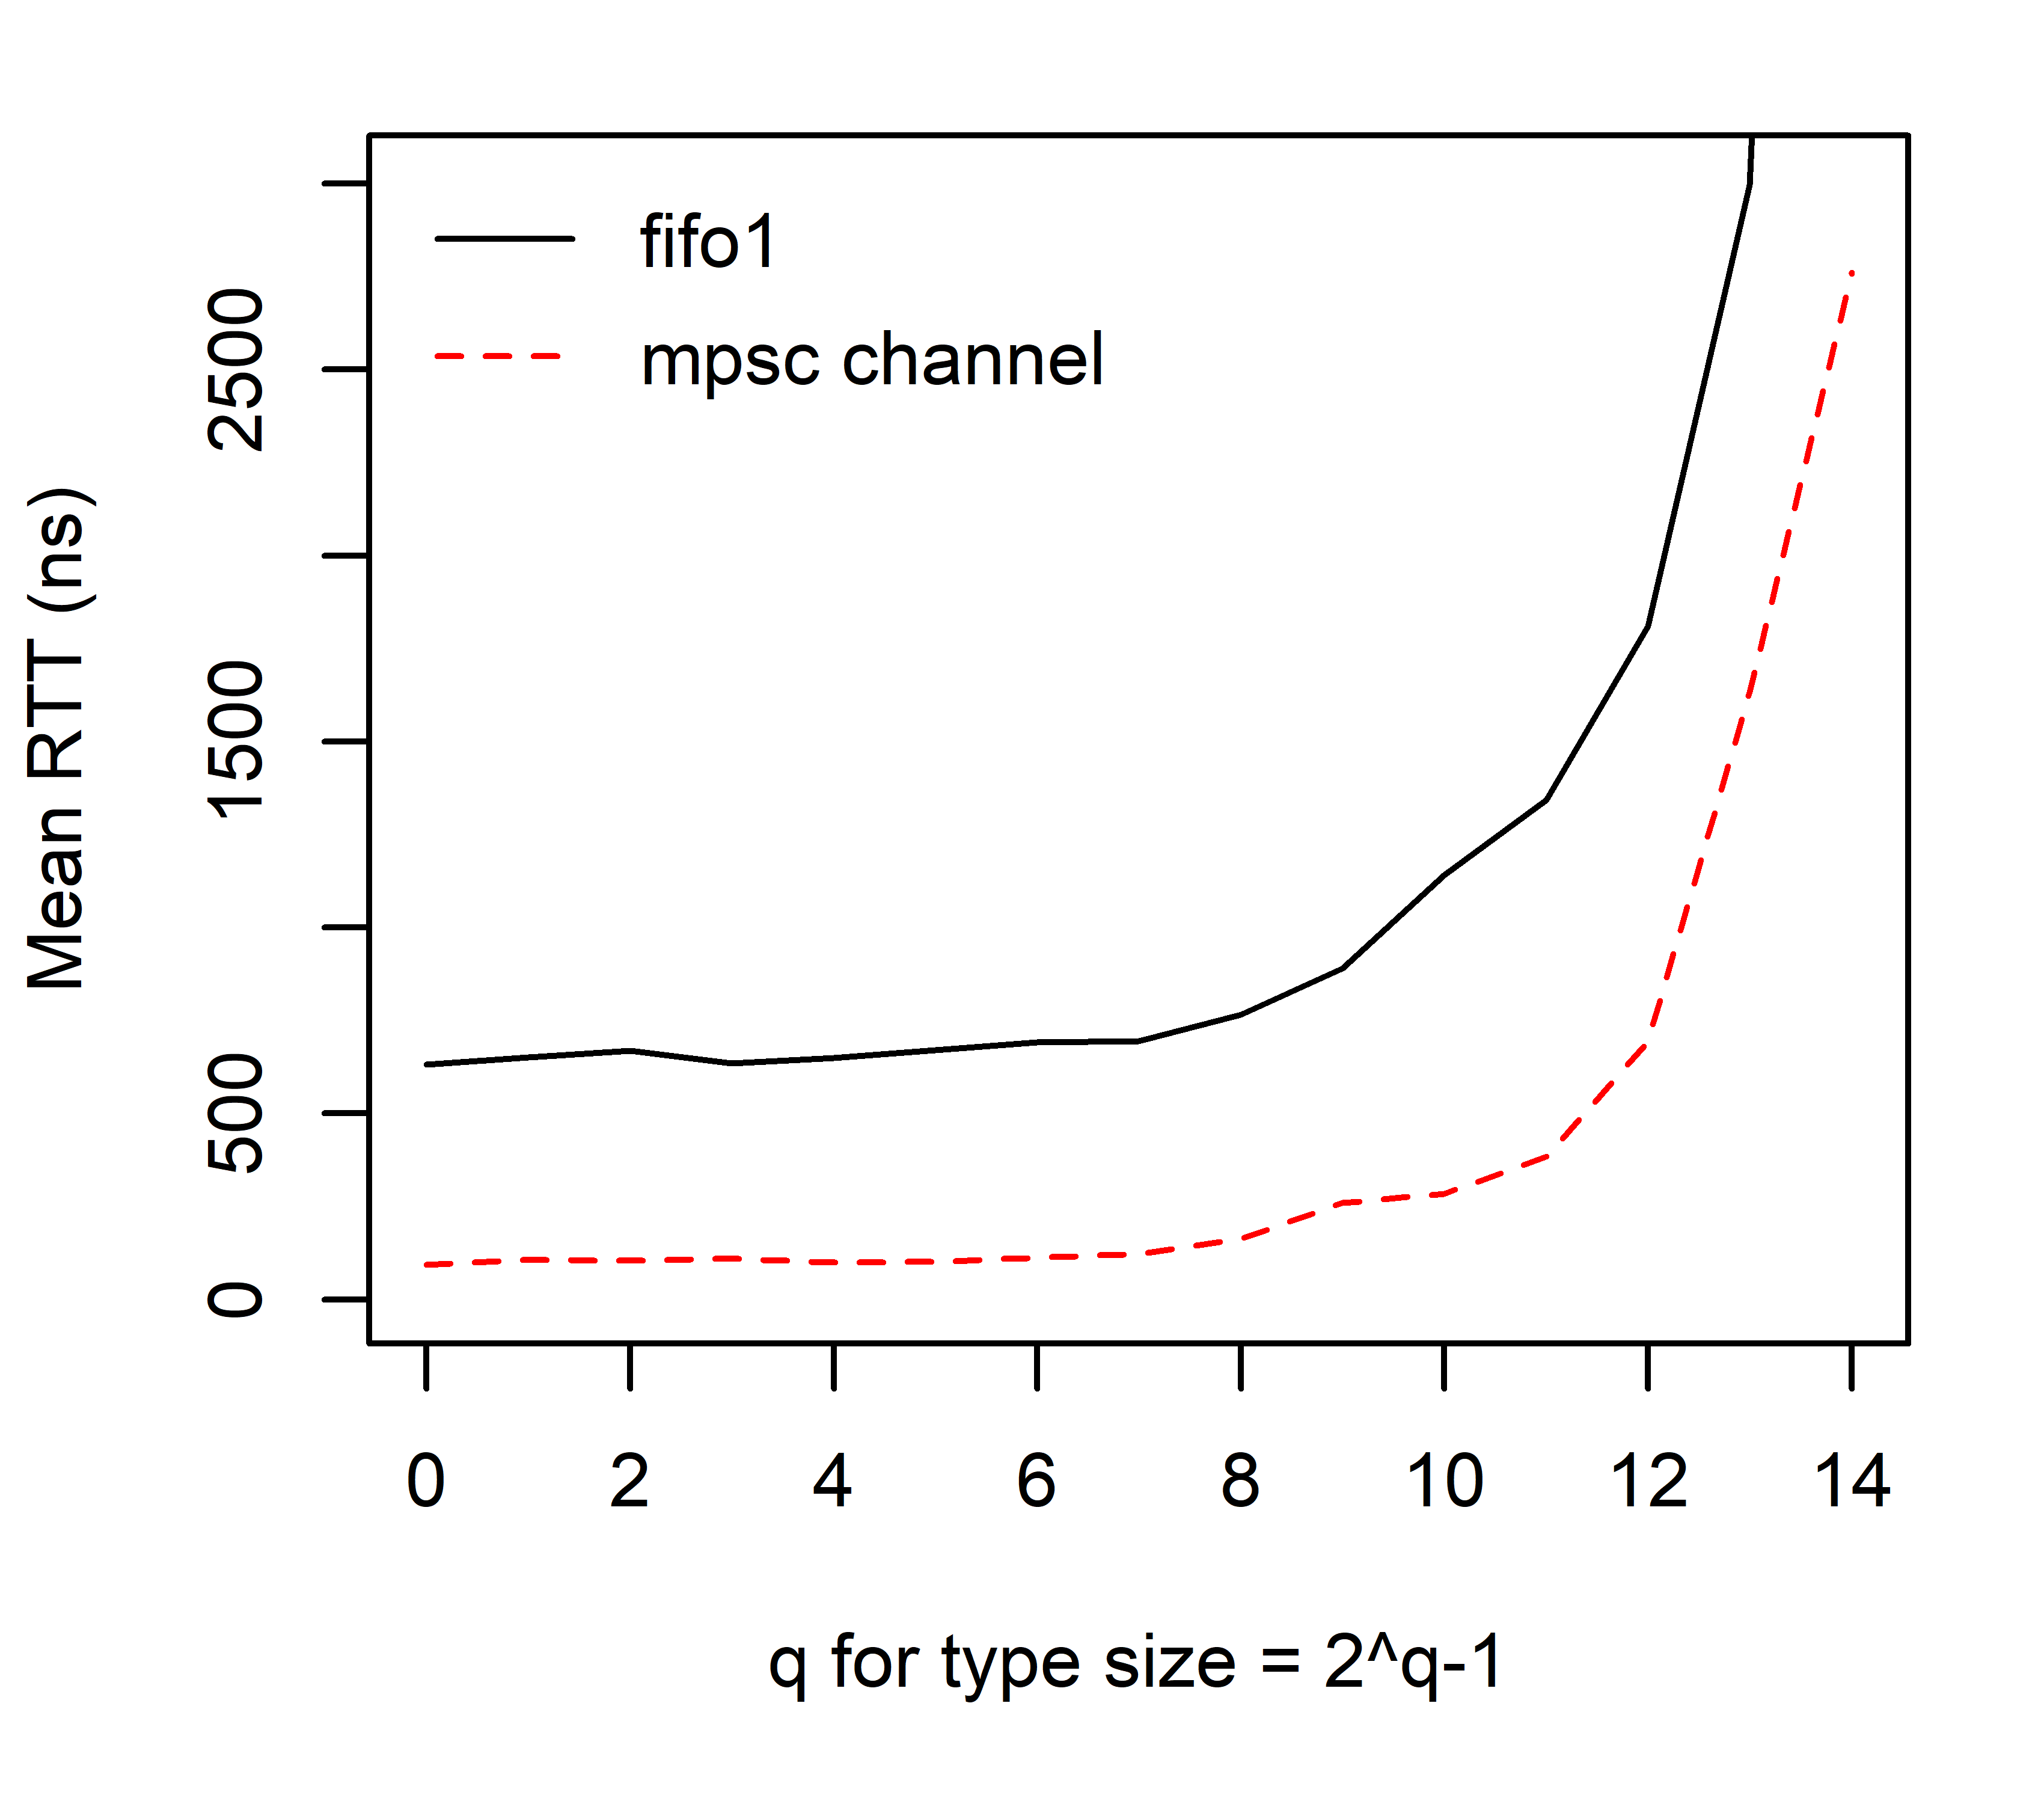
\includegraphics[width=\textwidth]{experiments/rtt_0.png}
			\caption{}
			\label{fig:exper_rtt_0}
		\end{subfigure}%
		\begin{subfigure}[b]{0.63\textwidth}
			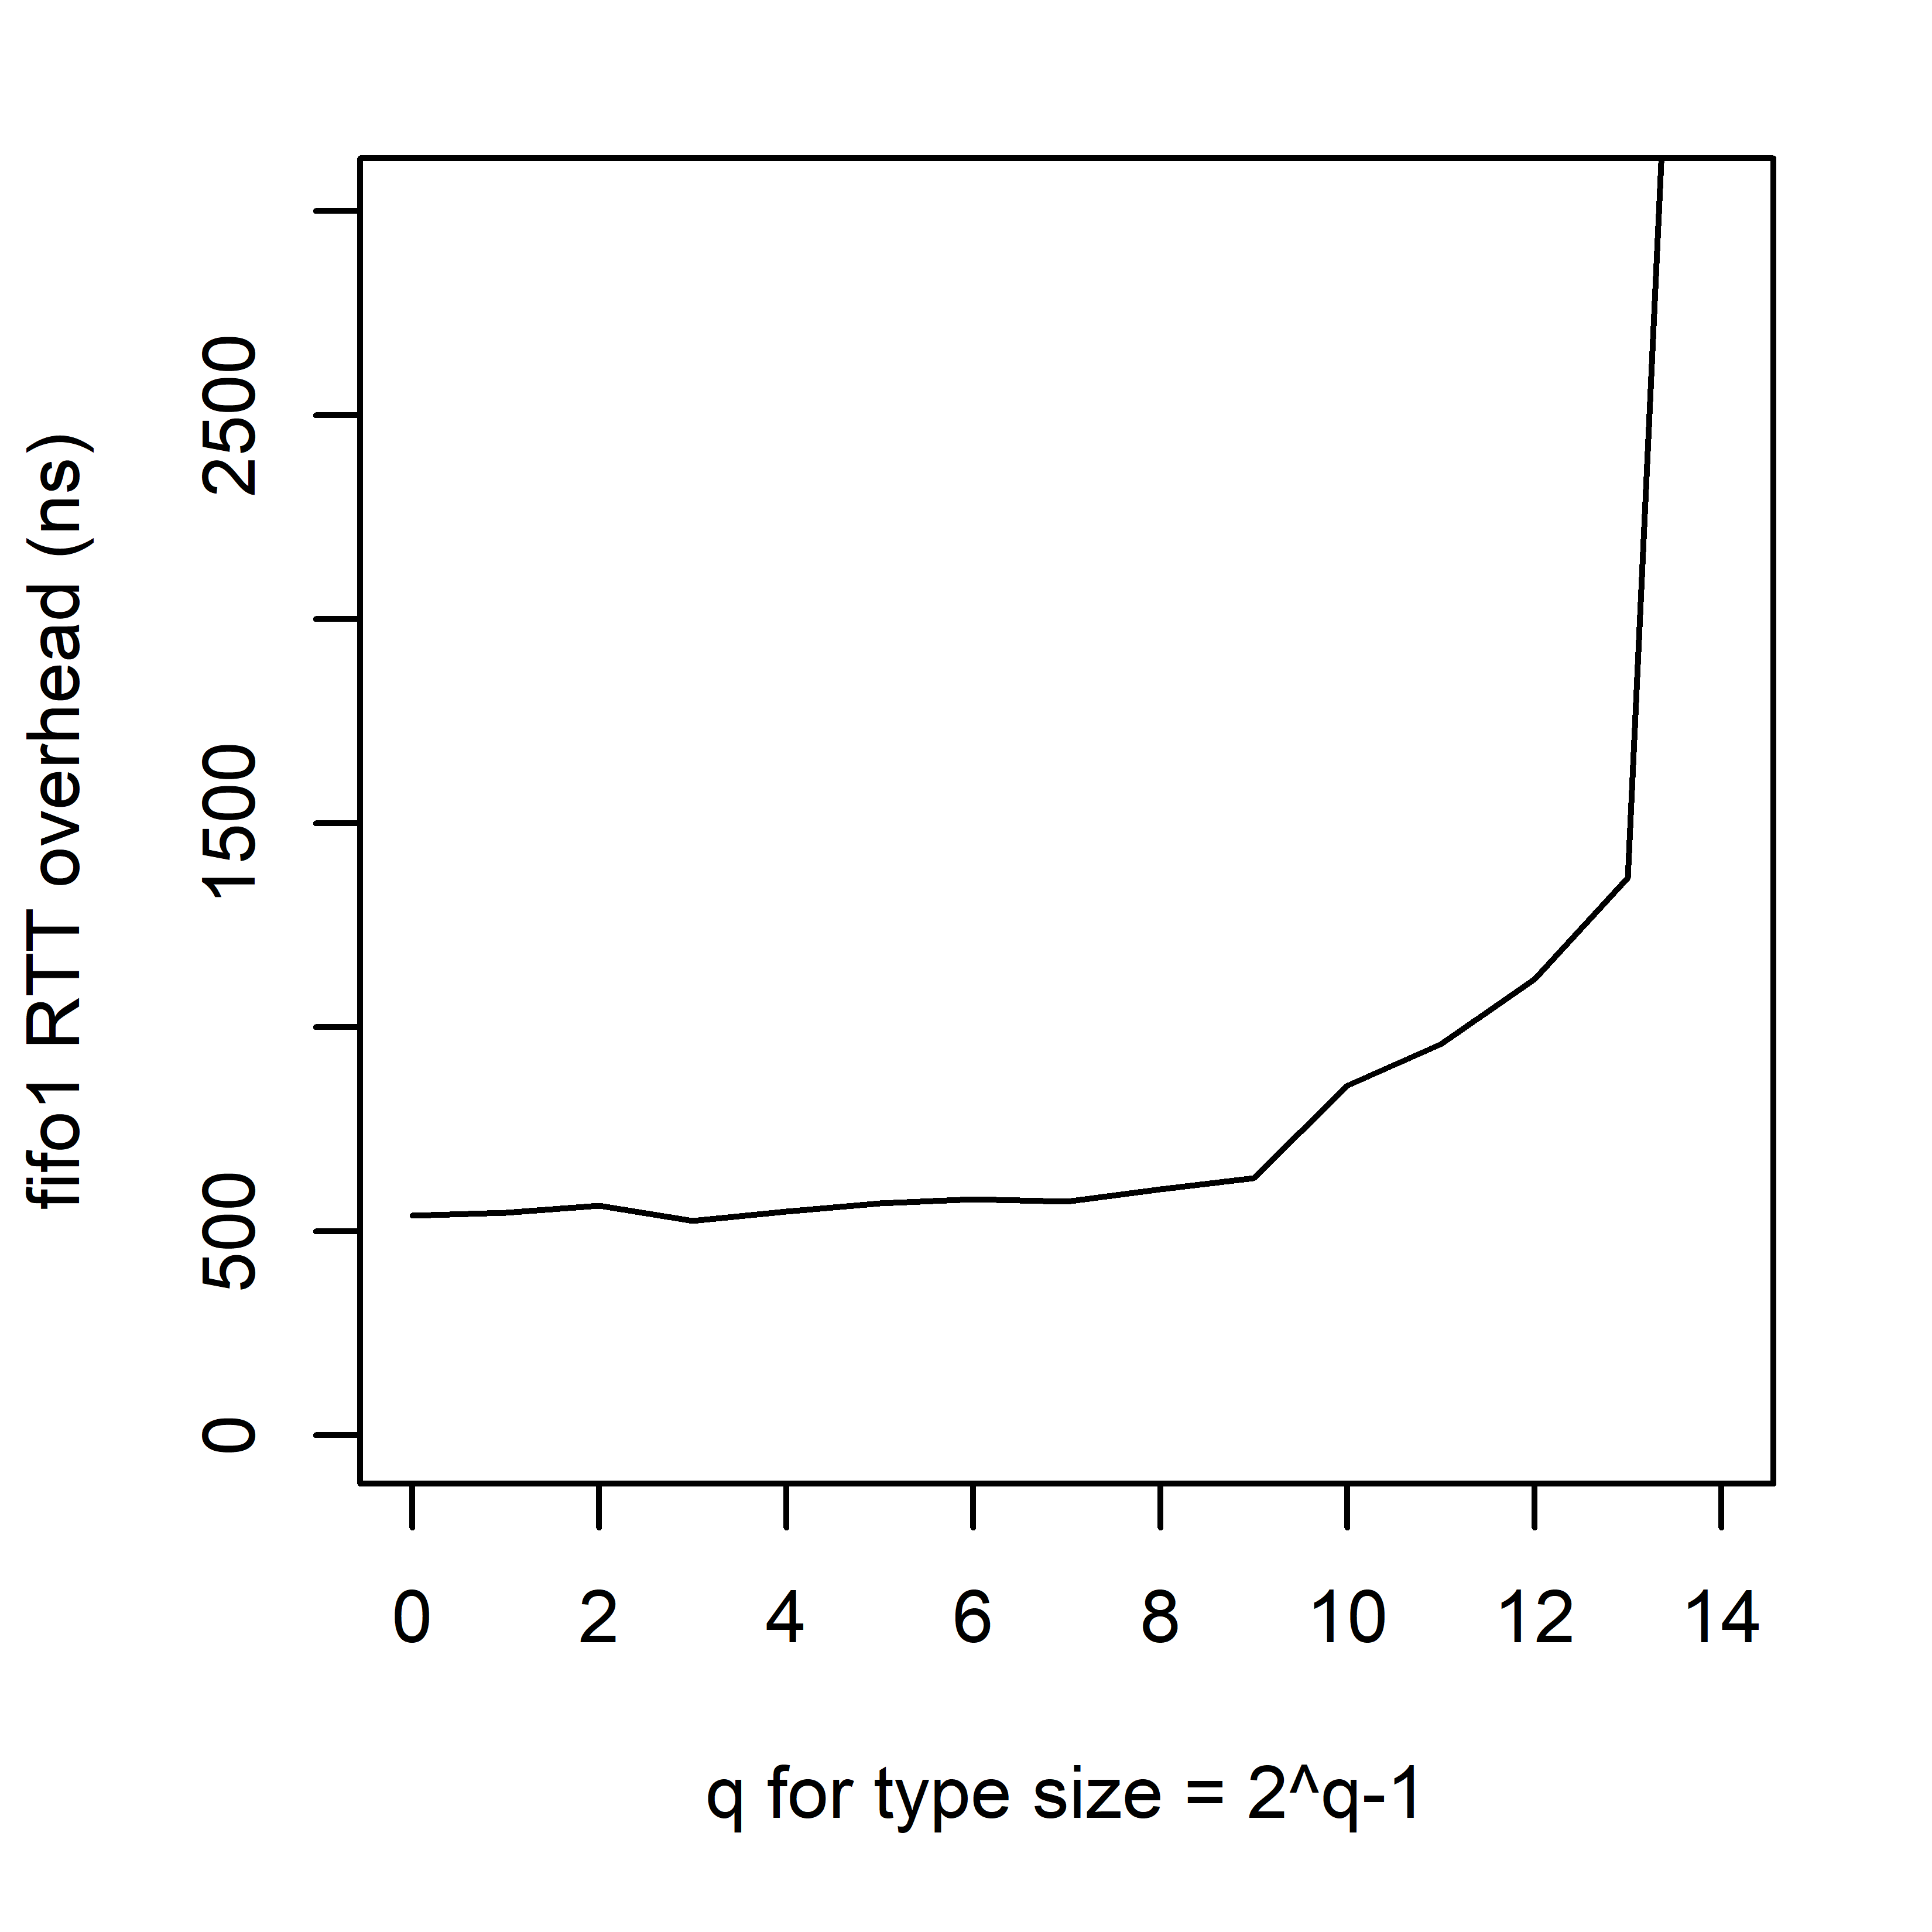
\includegraphics[width=\textwidth]{experiments/rtt_1.png}
			\caption{}
			\label{fig:exper_rtt_01}
		\end{subfigure}%
	}
	\caption[TODO]{Time from beginning of \code{put} to end of \code{get} in connector \textit{fifo1} compared to the time taken to send and received over an \code{mpsc} channel from the Rust standard library. Plots show the overhead in response to the size of the moved data. Figure~(b) shows the difference between the curves in Figure~(a), showing the overhead of Reo-rs more explicitly.}
	\label{fig:exper_rtt}
\end{figure}


These measurements show the range of times taken in response to changes in the data's size. The figure makes clear that compared to \code{mpsc}, Reo-rs experiences significant overhead in all cases. Some uniform overhead is to be expected, as \code{mpsc} is purpose-built and optimized for precisely this scenario. Reo-rs lacks the ability to optimize for this protocol to the same extent. For example, as explained in Section~\ref{sec:chosen_design}, all port-operations involve the acquisition of a shared protocol lock. Conceptually, Reo-rs has all the information it needs optimize for this protocol and particular and match the performance of \code{mpsc}. The generality of Reo-rs inhibits its ability to identify and specialize for these kinds of optimizations to the same extent as was done by hand for \code{mpsc}. A hand-optimized fifo1 channel could take advantage of the fact that the two ends of the channel need not share a lock at all. For this protocol, partitioning the coordinator such that each part only considers \textit{local} rules would be correct and cause less contention.

Figure~\ref{fig:exper_rtt_01} makes clear that Reo-rs is experiencing overhead that increases with the size of the moved value. At first glance, one can be forgiven for attributing this overhead to the presence of redundant movements of the data, which Section~\ref{sec:port_operations} explains can occur if llvm fails to optimize away the \textit{physical} movements from Rust's \textit{semantic} movements of values to new variable bindings. This turns out not to be the cause in this case. Rather, the overhead is caused by a more granular implementation detail; \code{mpsc} has a different method of moving its values. Listing~\ref{listing:mpsc_pop} gives a glimpse into how \code{mpsc} has some means to optimize data movements in the case of an x86-64 processor by `in-lining' it, spelling it out into a sequence of smaller movements hundreds of lines long. In this manner, \code{mpsc} is optimized to avoid the overhead of system calls.

\begin{listing}[h!]
	\centering
	\inputminted{text}{mpsc_pop.txt}
	\caption[TODO]{TODO}
	\label{listing:mpsc_pop}
\end{listing}

For connectors as simple as \textit{fifo1}, overhead is overhead. However, we are particularly interested in understanding how this overhead is partitioned; as connectors become more complex, different parts of this overhead impact \textit{parallelism} in different ways. Section~\ref{sec:protocol_runtime} explains the nature of the \textit{coordinator} role, and how its operations are performed holding the lock for the \code{Proto} instance which connects ports as their common communication medium. Table~\ref{tab:active_time} shows measurements for an experiment that attempts to understand which proportion of our overhead is incurred \textit{inside} the critical region, ie.\ by the coordinator. In the case of this experiment, our protocol has rules for movement which can be rendered as a \textit{bipartite graph}, allowing data flow from any putter in $\{P0, P1, P2\}$ to any getter in $\{G0, G1, G2\}$. As explained in Section~\ref{sec:data_exchange}, movements such as these do not buffer the data elements inside the protocol; getters take values from putters directly. As a consequence, putters are both the first and last to parttake in any of our rule firings' data movements. The table shows the mean duration for which each putter was involved in such a firing. Along with the total duration of the run, we are able to compute to which extent these putters were able to work in parallel. We distinguish between four cases, corresponding to rows in Table~\ref{tab:active_time}. The first three cases do not involve the \code{clone} operation, and are observed to have insignificant differences for all measurements. For this experiment, with modestly-sized values, we conclude that there is no large difference in performance between these three cases:
\begin{enumerate}
	\item [\textbf{move}] Values are moved from putter to getter synchonously.
	\item [\textbf{copy}] Putters retain their values, and getters replicate them with a bit-wise copy that does not mutate the original.
	\item [\textbf{signal}] Getters do not return any data. They return after releasing putters.
\end{enumerate}

The final \textbf{clone} case attempts to observe the effects of intentionally delaying getters outside of the lock by necessitating the use of an explicit \code{clone} operation whose duration is artificially lengthened\footnote{At these small timescales, \code{sleep} calls were out of the question, as their variance from the requested duration would drown out our other measurements. Instead, clone is implemented for our type to replicate the original and then perform thousands of chaotic integer computations on the replica before returning it. This operation was chosen to be intentionally obtuse such that the Rust compiler is unable to identify a trivializing optimization.}. For these runs, putters retained their original values, but the datum was not marked with the \code{Copy} trait. In all cases, we observed that even at this coarse granularity, there was significant parallelism. For the majority of the time, new rules were able to fire whilst interactions were being completed outside of the critical region. The final case in particular was within a small rounding error of perfect parallelism.

\begin{table}[]
	\begin{tabular}{l|lll|ll}
		& \multicolumn{3}{l|}{mean active time} & \multirow{2}{*}{\begin{tabular}[c]{@{}l@{}}run\\ duration\end{tabular}} & \multirow{2}{*}{\begin{tabular}[c]{@{}l@{}}mean\\ parallelism\end{tabular}} \\
		& p0 & p1 & p2 &  &  \\ \hline
		move & 2.037µs, & 2.031µs, & 2.017µs & 214.991ms & 2.83 \\
		copy & 1.744µs, & 1.852µs, & 1.844µs & 197.676ms & 2.75 \\
		signal & 1.962µs, & 1.956µs, & 1.937µs & 207.181ms & 2.83 \\
		\hline
		clone & 94.021µs, & 94.082µs, & 94.058µs & 9420.148ms & 2.995 
	\end{tabular}
	\caption[TODO]{TODO}
	\label{tab:active_time}
\end{table}

\subsection{Coordination}
Its important to understand what the coordinator is spending time on, as this is the bottleneck to concurrency. 
Figure~\ref{fig:check_time} gives an overview of how long various non-firing rules add to the coordination time. here we see the round trip from the moment get is initiated to the moment it completes in a situation where always one rule can fire. we have designed it such that a number of blocked rules are always evaluated first. here we plot the time taken for each of these connectors, plotted over the number of these bogus rules encountered. we observe the expected linear scaling. The time for 0 bogus rules clearly shows the NON overhead time. non-ready guards cost 8.76 nanosec, false checks cost 18.91 ns each, 5x5 nested and checks were 180.72 each, allocations were 316.51 ns each, including freeing etc. 
\begin{figure}
	\centering
	\makebox[\textwidth][c]{
		\begin{subfigure}[b]{0.63\textwidth}
			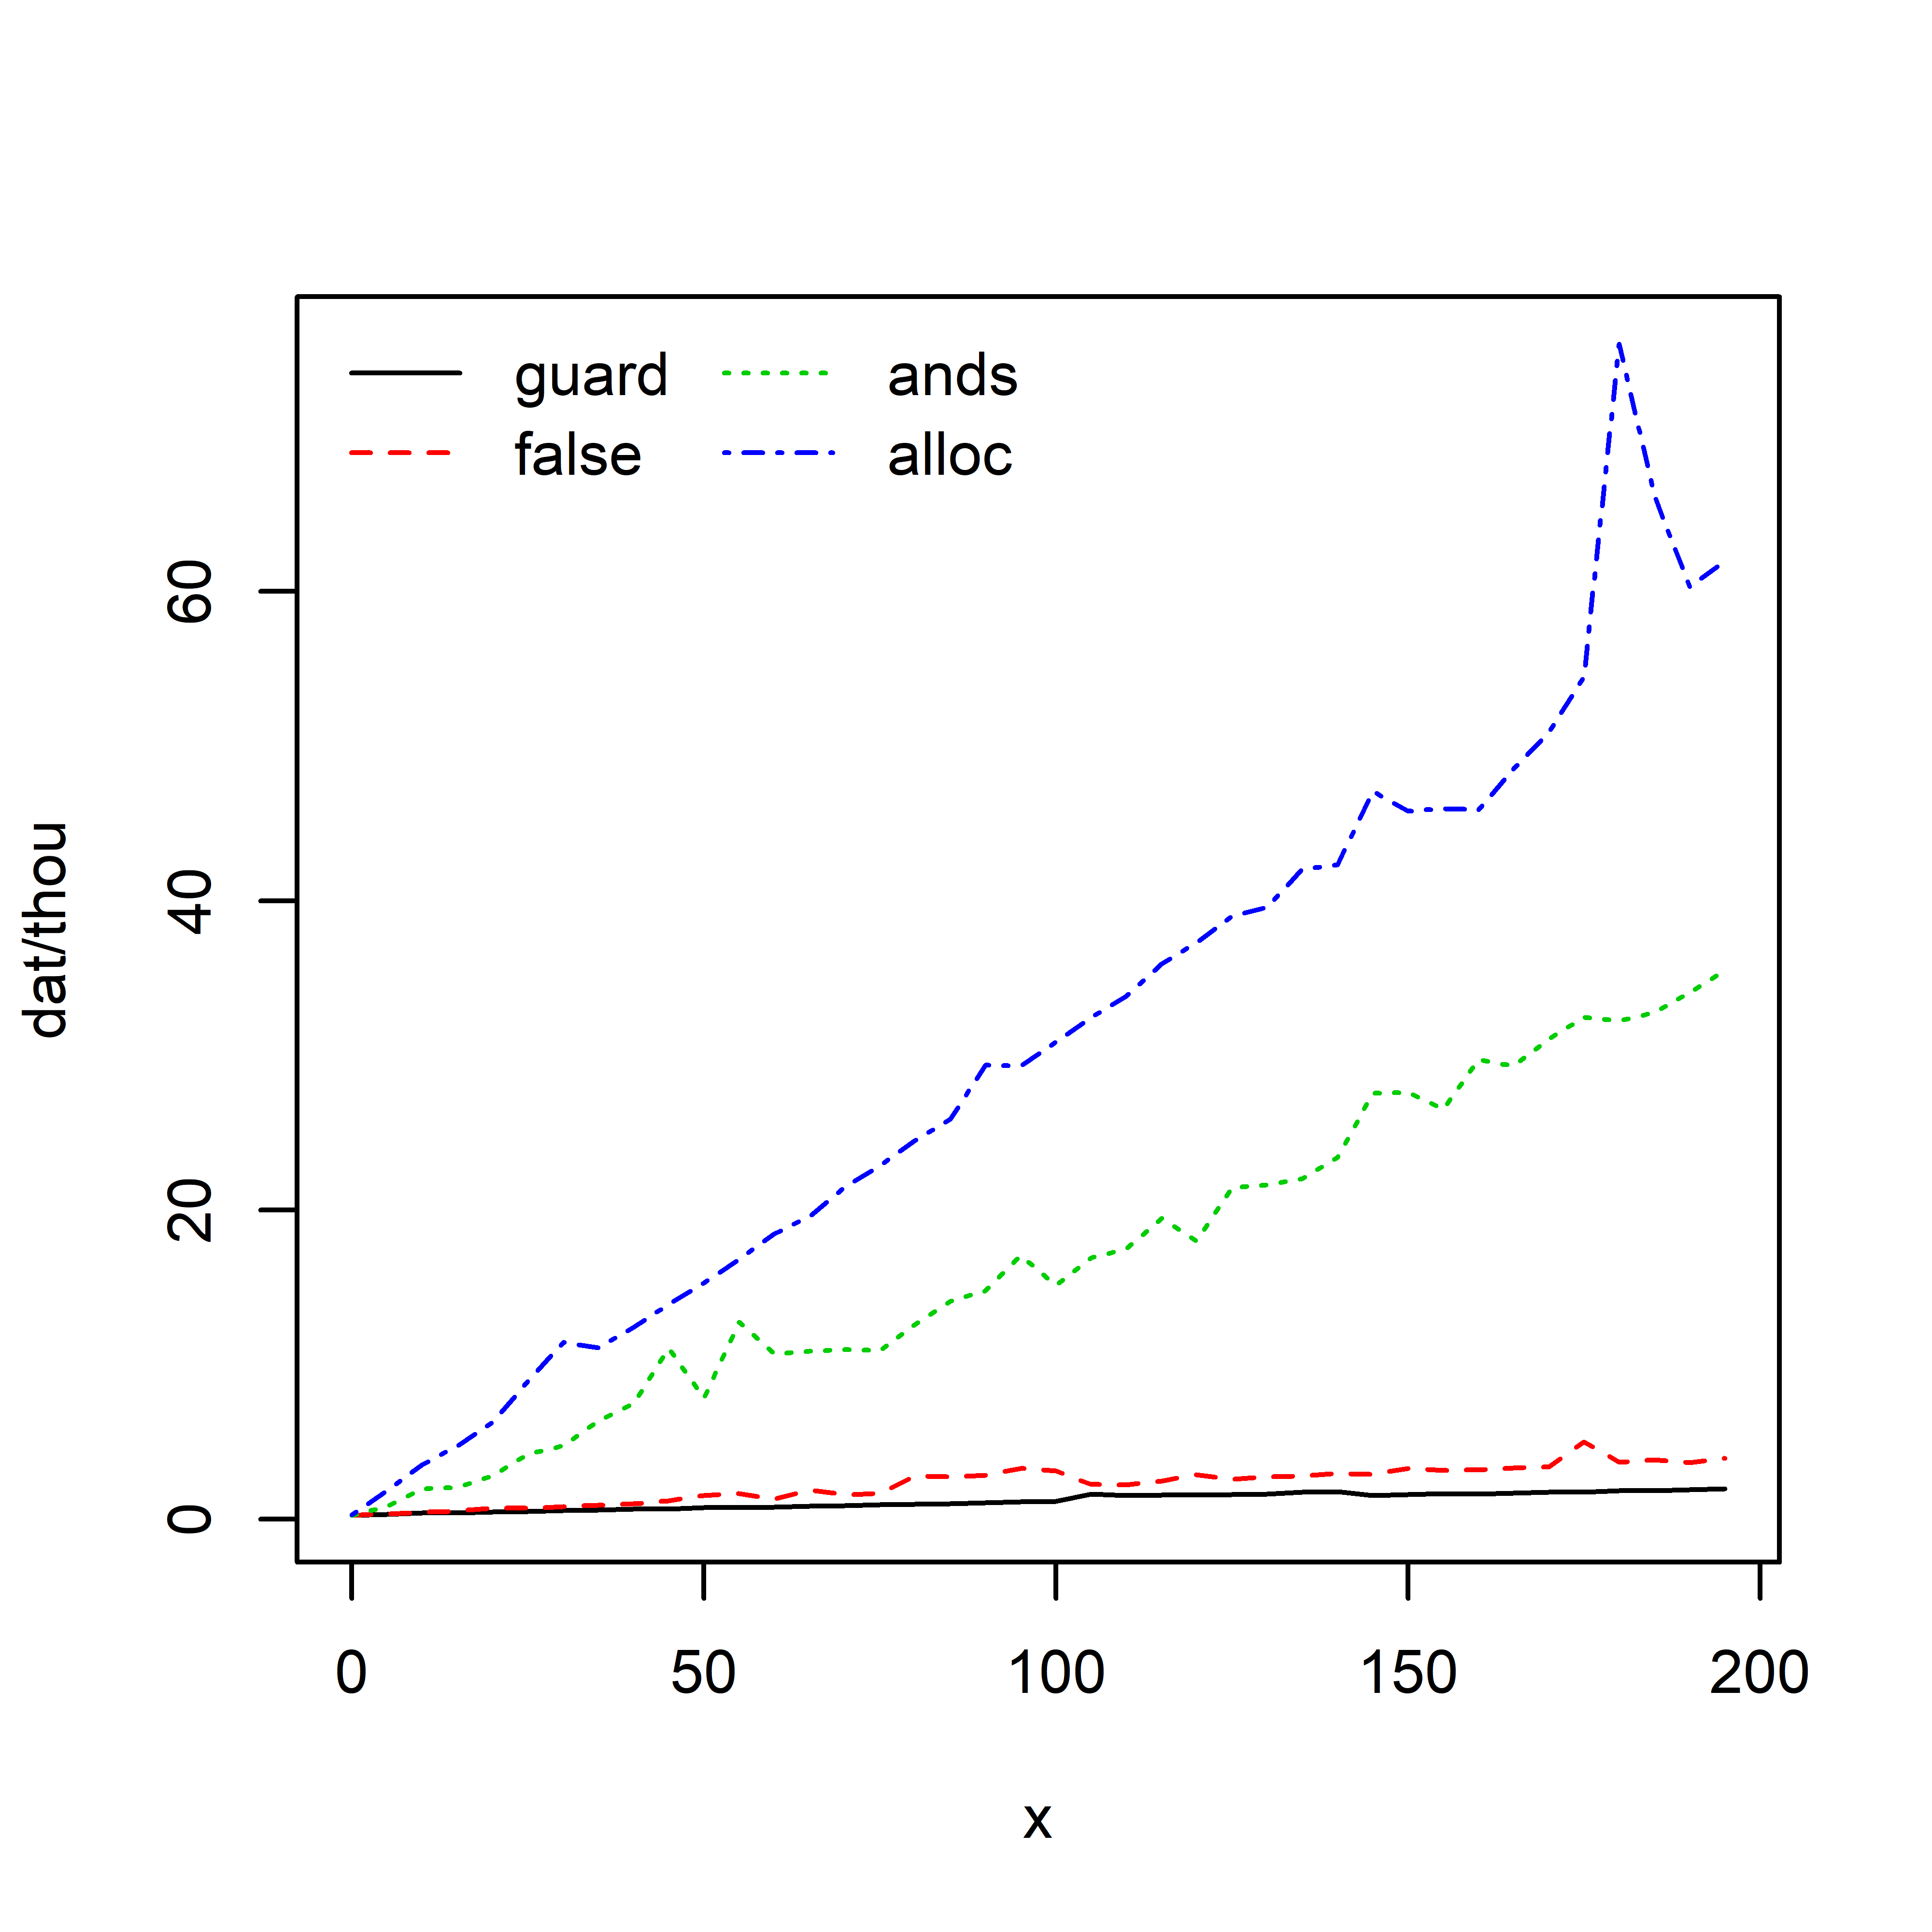
\includegraphics[width=\textwidth]{experiments/check_time_0.png}
			\caption{}
			\label{fig:check_time_0}
		\end{subfigure}%
		\begin{subfigure}[b]{0.63\textwidth}
			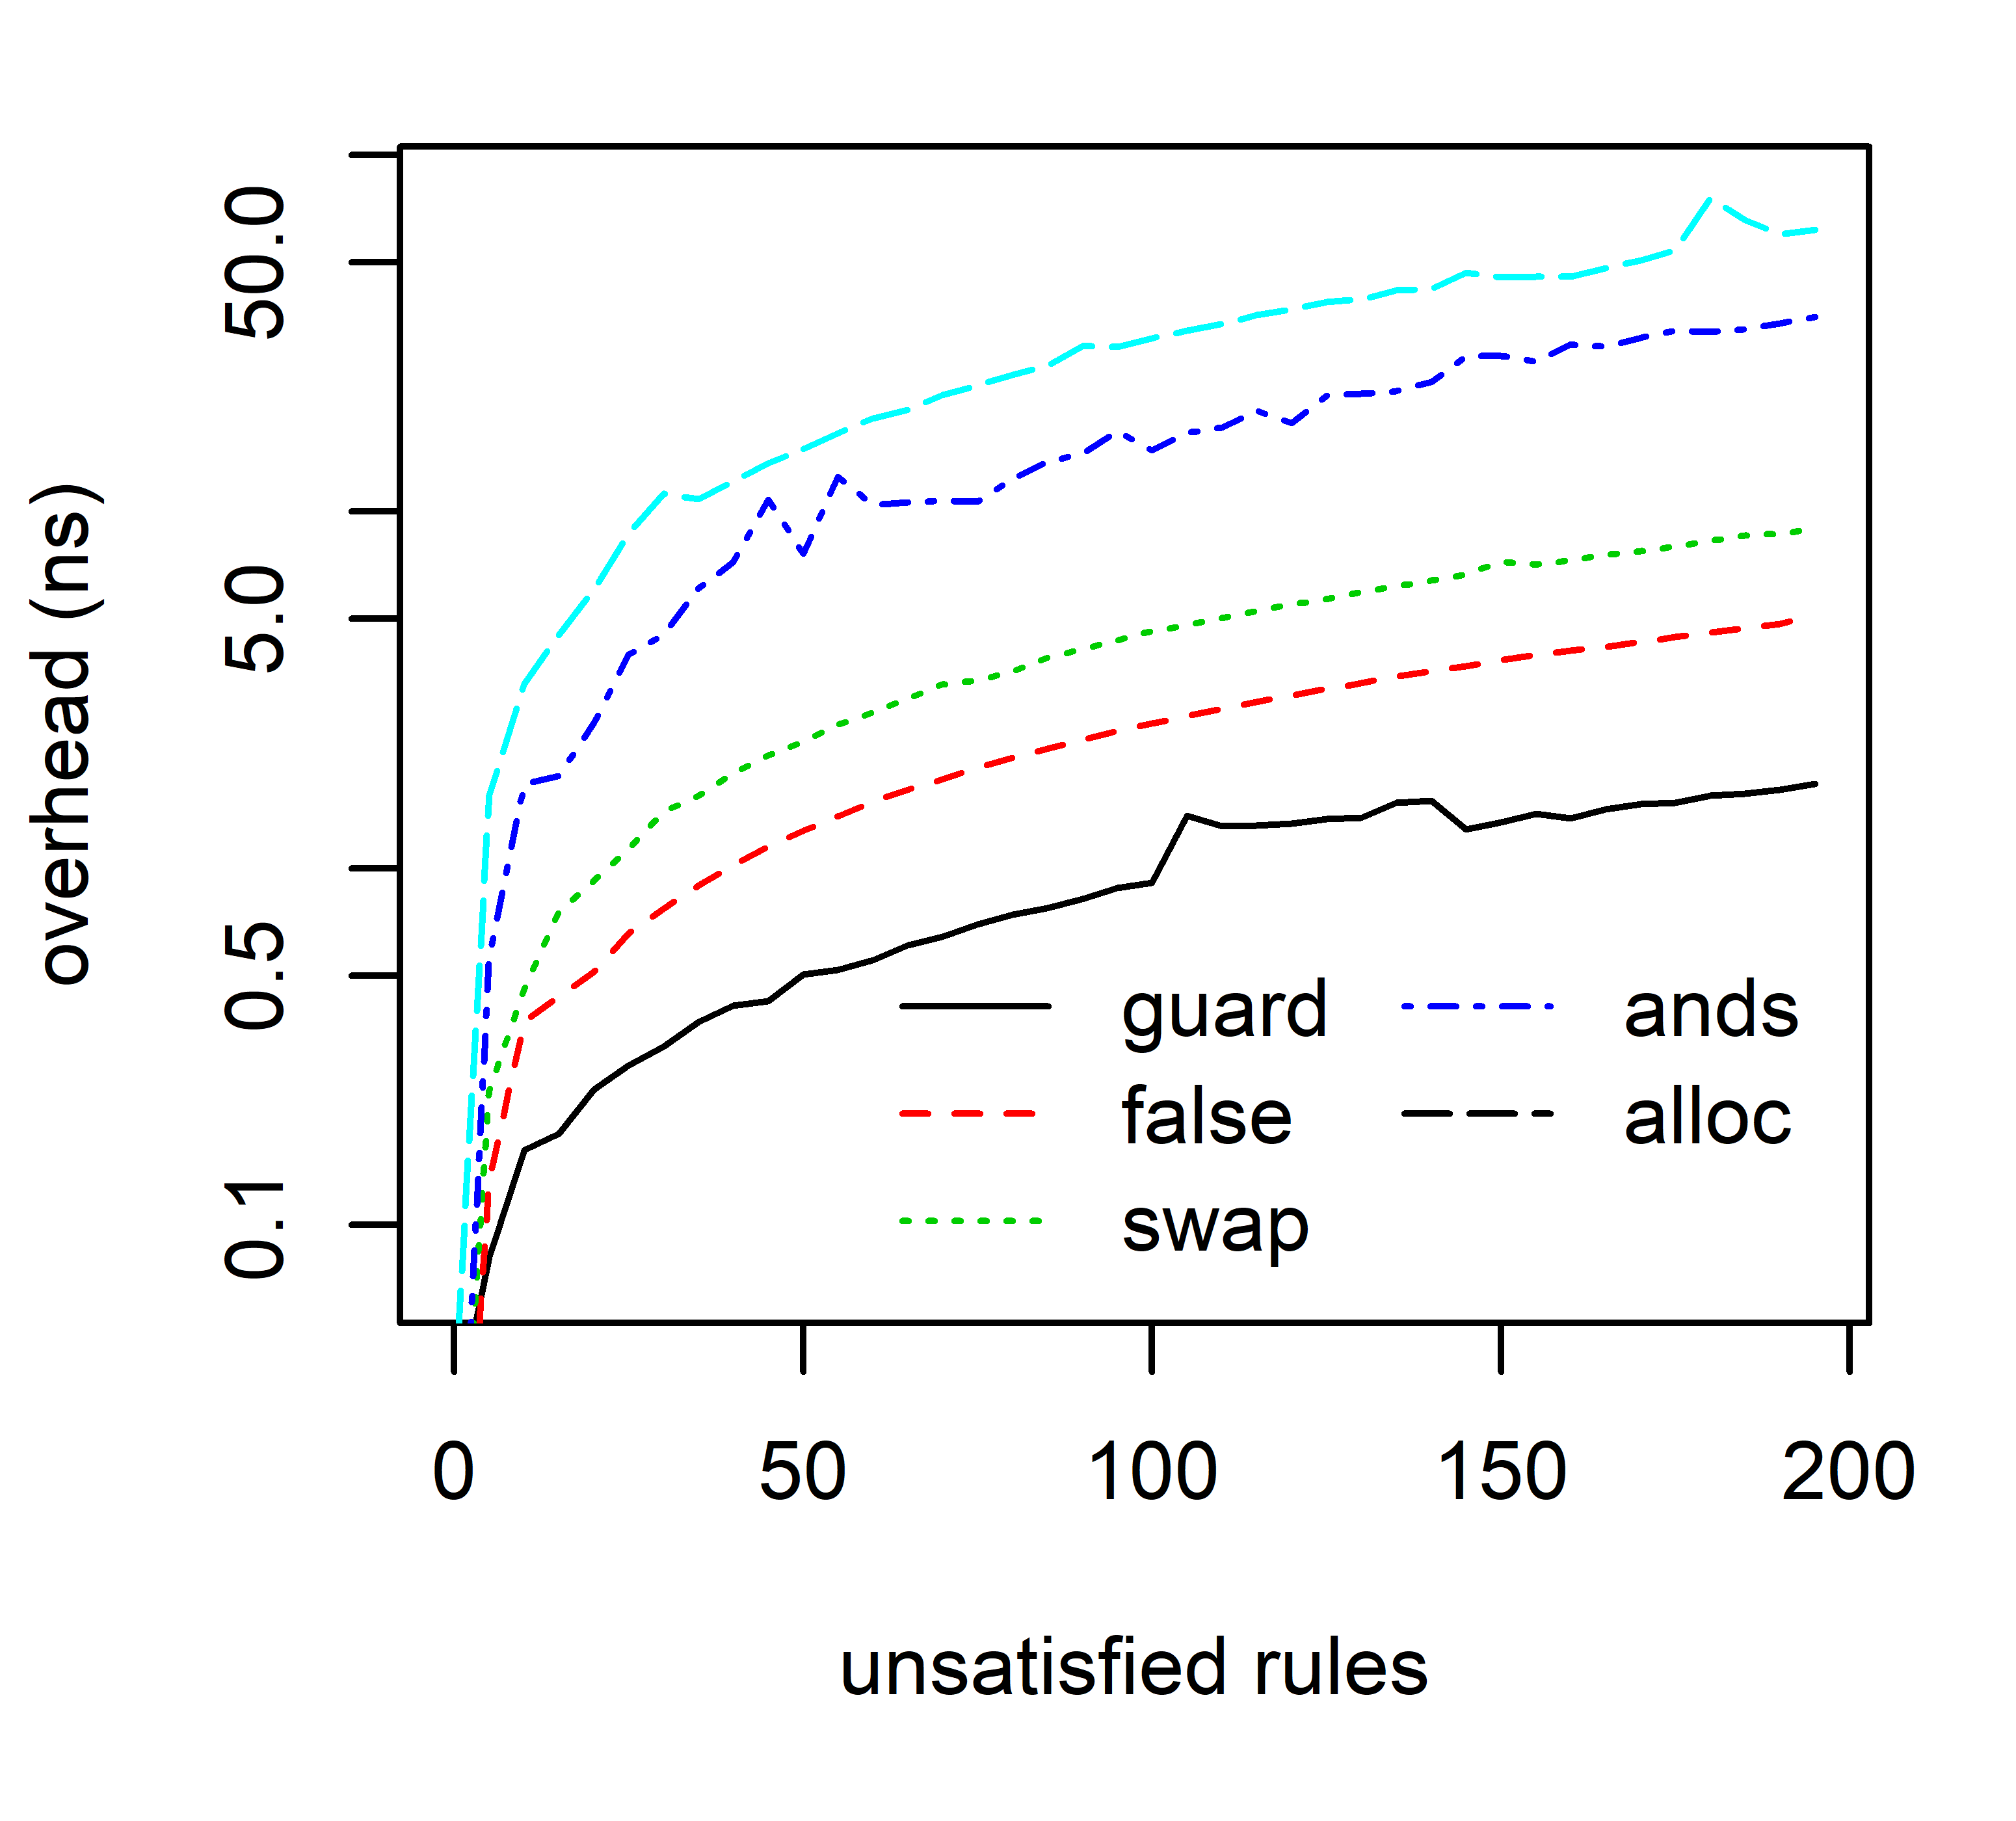
\includegraphics[width=\textwidth]{experiments/check_time_1.png}
			\caption{}
			\label{fig:check_time_2}
		\end{subfigure}%
	}
	\caption[TODO]{TODO.}
	\label{fig:check_time}
\end{figure}

\subsection{Data Exchange}
So what about the overhead outside the lock? inside the movements themselves. We measure the time taken for a group of getters to get from a single putter in response to data of different sizes (this influences the cost of COPYING)




We examine the operation which usually contributes most to the cost of a movment: cloning. we check what happens when the 
Figure~\ref{fig:clone_compete} shows how long interactions take with N getters with a value that cannot be copied. observe the large jump from 1 to 2, as one is the mover. effectively when there is only one getter, no cloning is necessary. When the single-getter case is ignored, we see that larger numbers of getters converge on a ratio of time taken = 1 the larger the data, seen in Figure~\ref{clone_compete_3}. The cost of the clone operation itself is controlled. 10k work units takes 2.4 microsec (TODO) not including dynamic dispatch etc
\begin{figure}
\centering
\makebox[\textwidth][c]{
	\begin{subfigure}[b]{0.63\textwidth}
		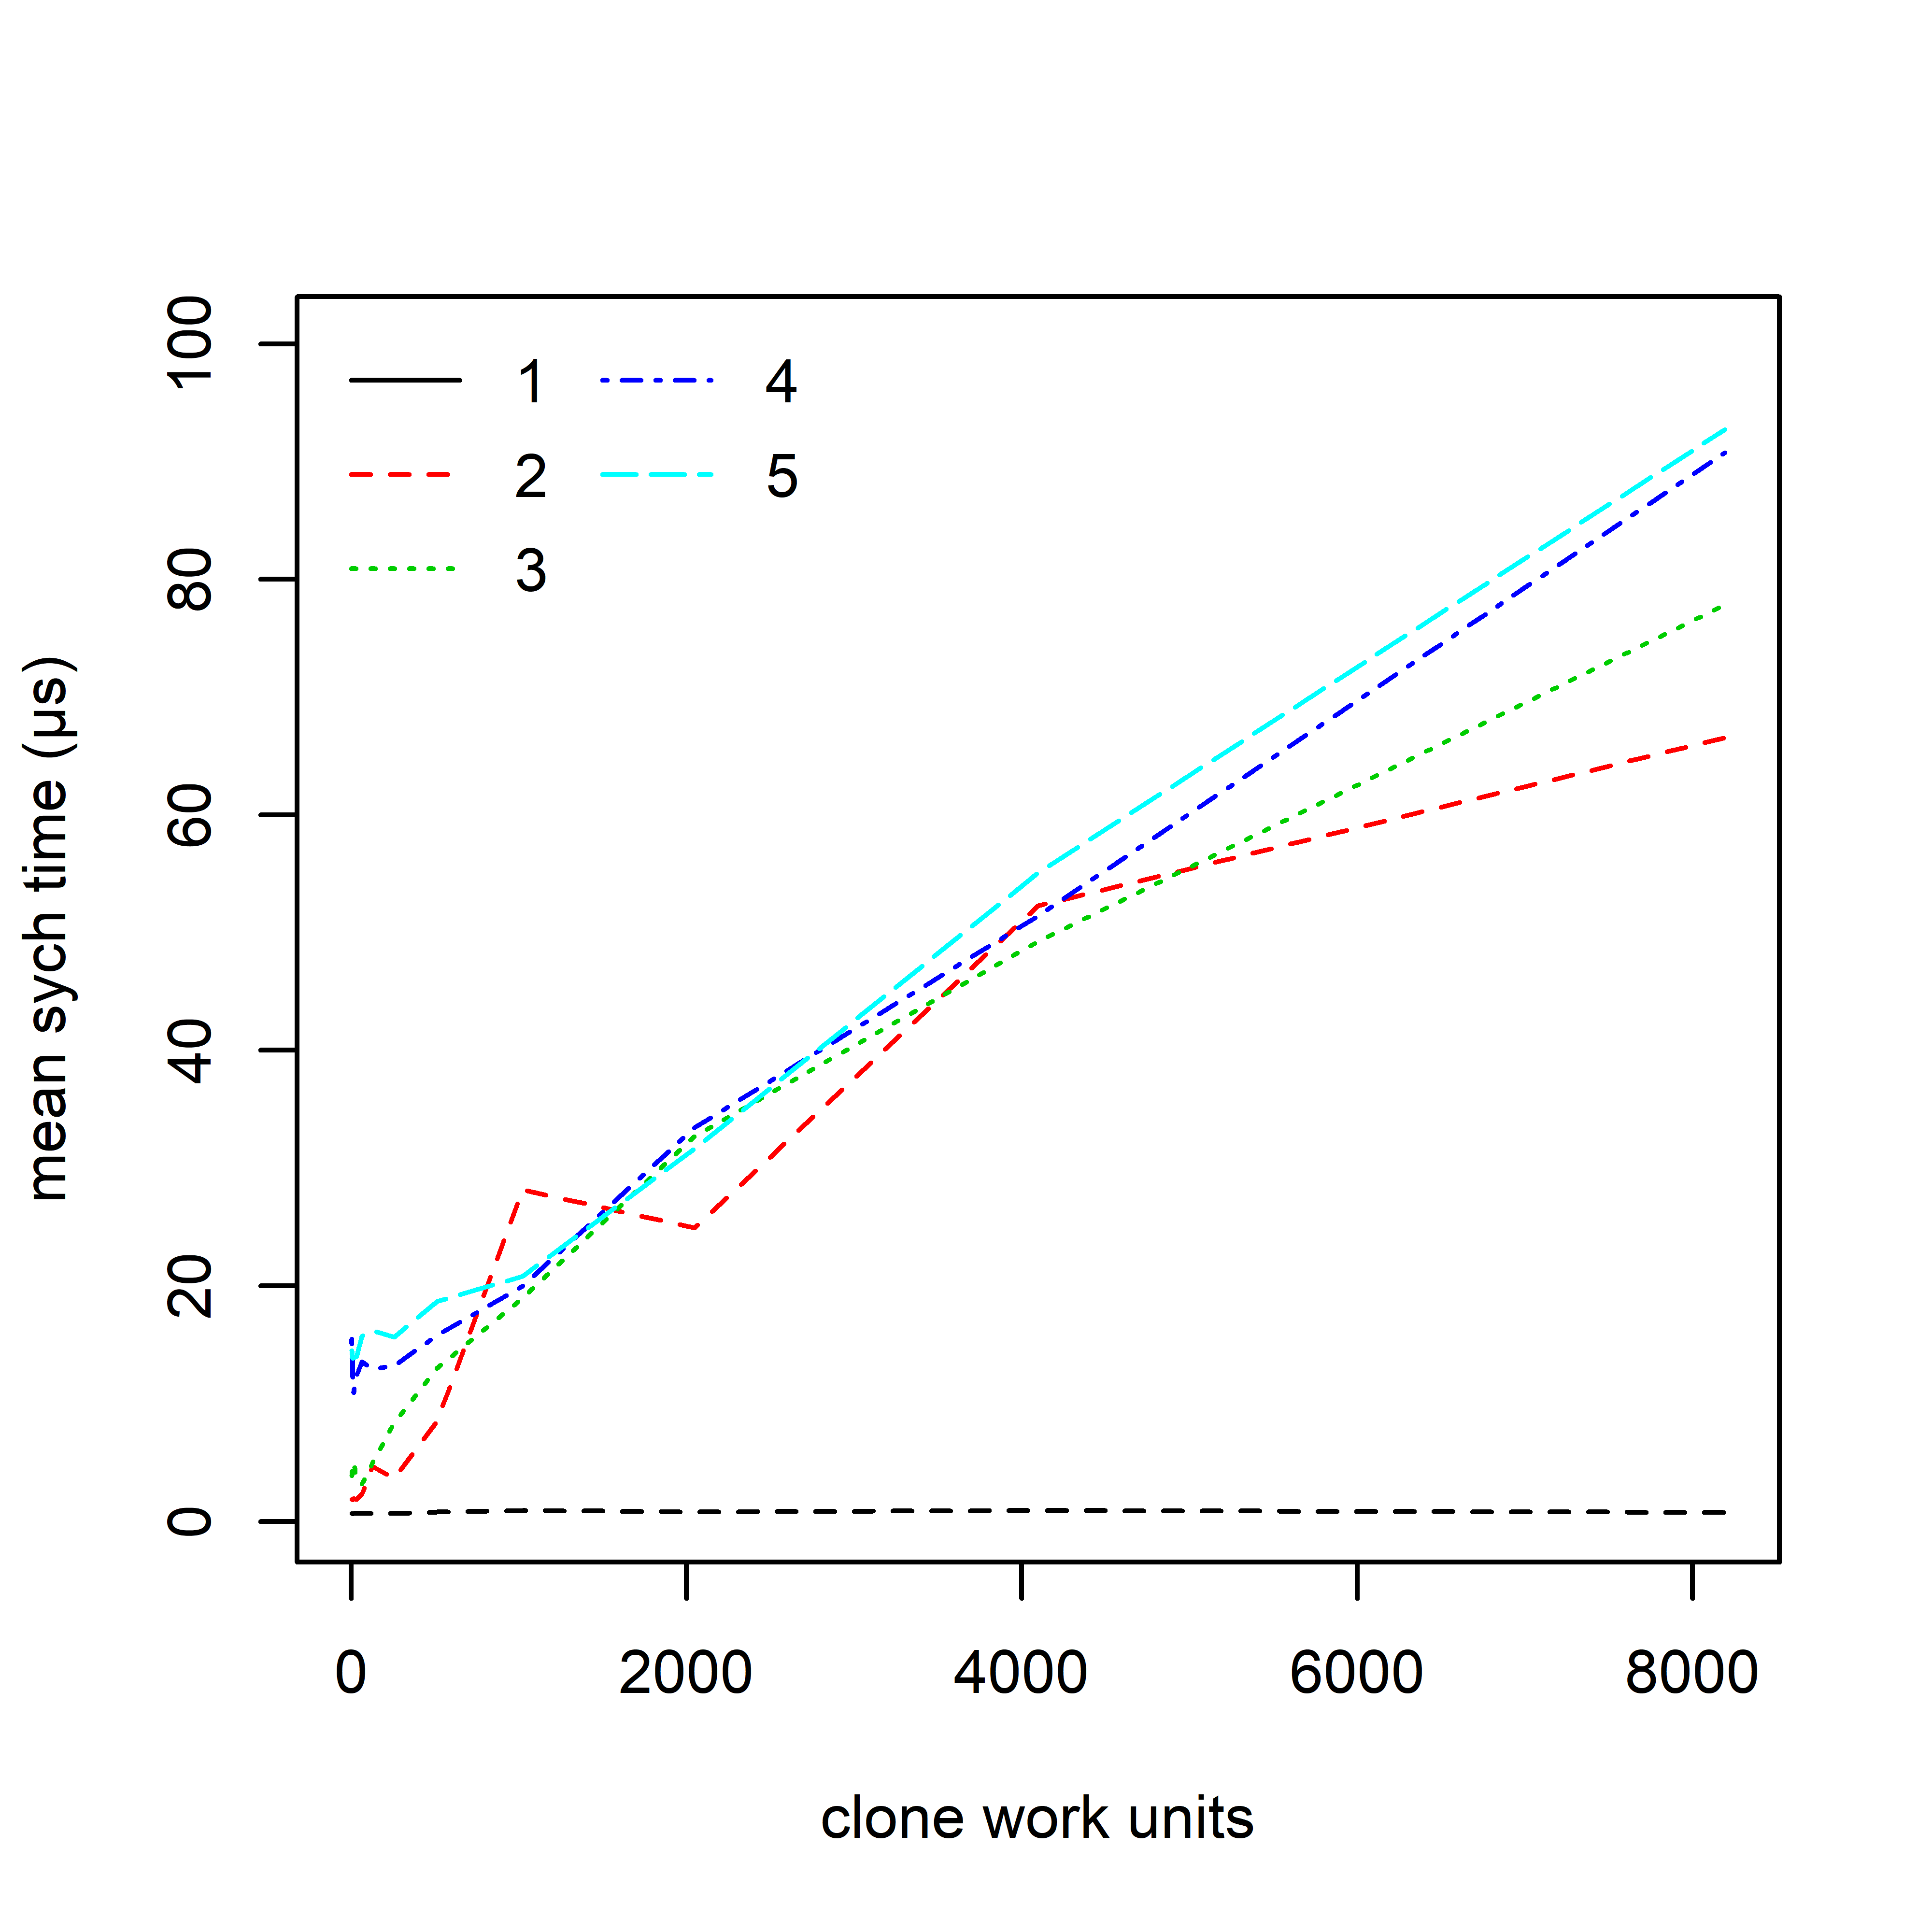
\includegraphics[width=\textwidth]{experiments/clone_compete_0.png}
		\caption{}
		\label{fig:clone_compete_0}
	\end{subfigure}%
	\begin{subfigure}[b]{0.63\textwidth}
		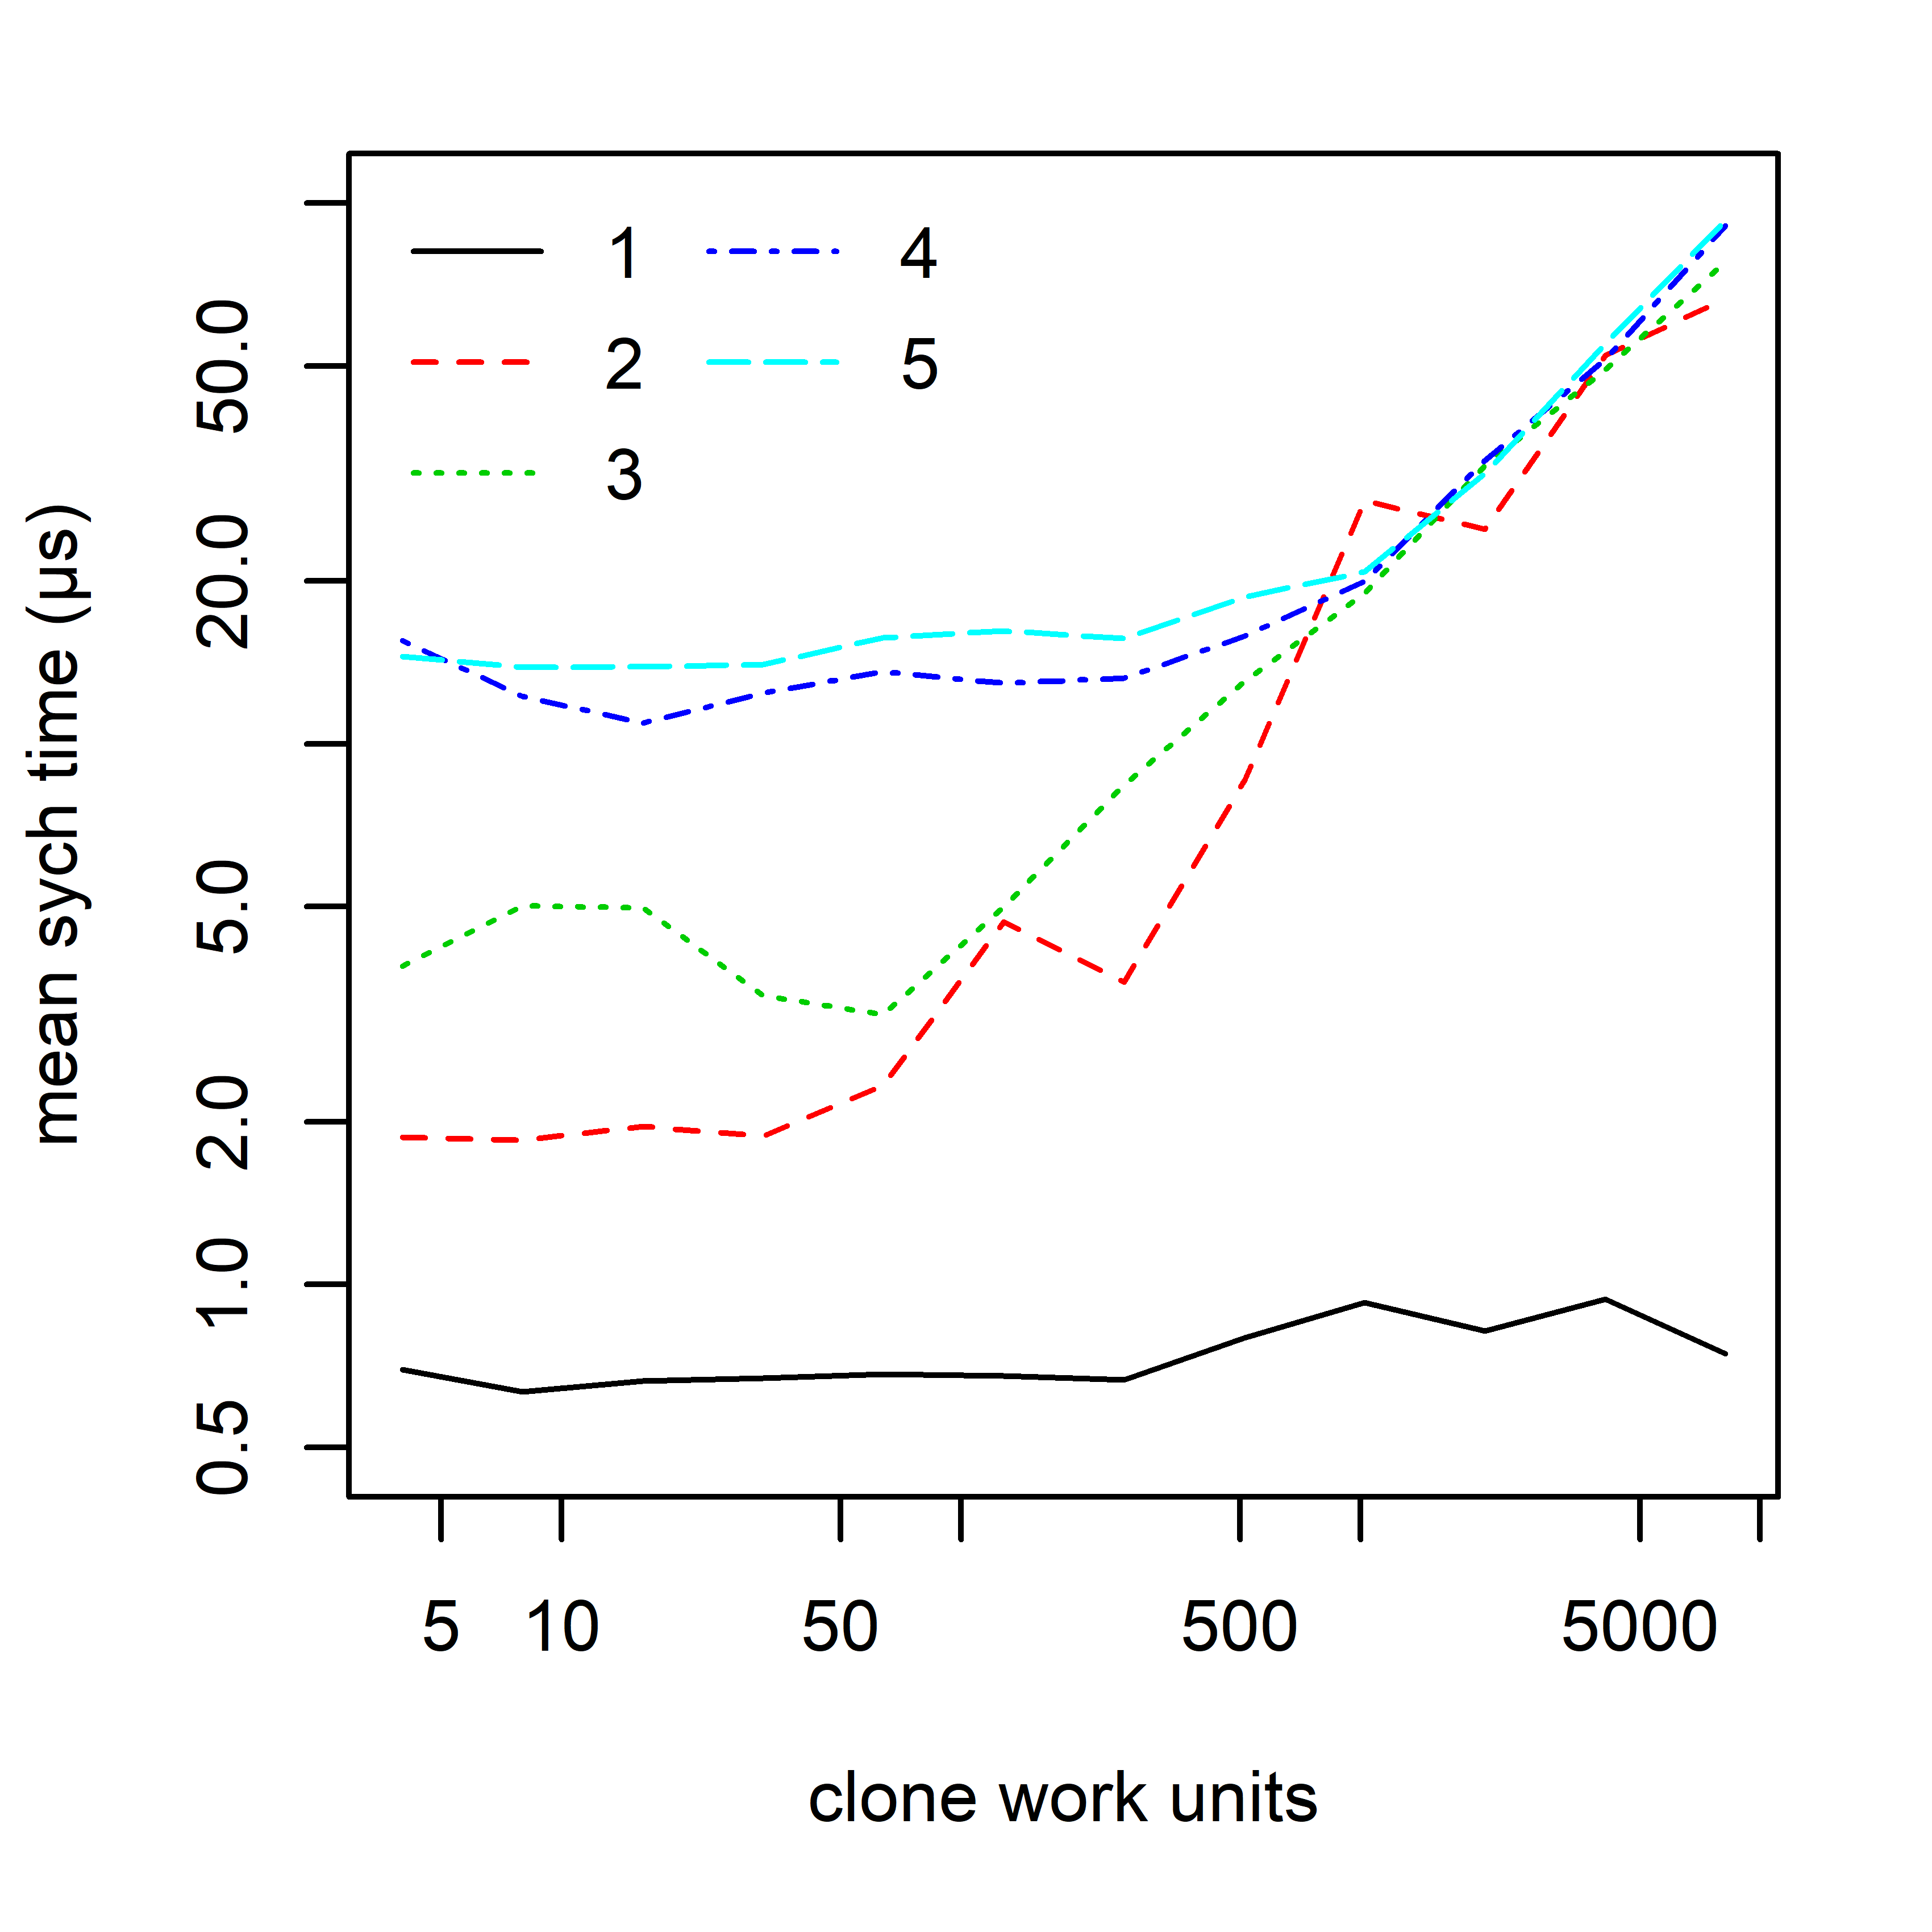
\includegraphics[width=\textwidth]{experiments/clone_compete_1.png}
		\caption{}
		\label{fig:clone_compete_1}
	\end{subfigure}%
}
\caption[TODO]{TODO.}
\label{fig:clone_compete}
\end{figure}

\begin{figure}
	\centering
	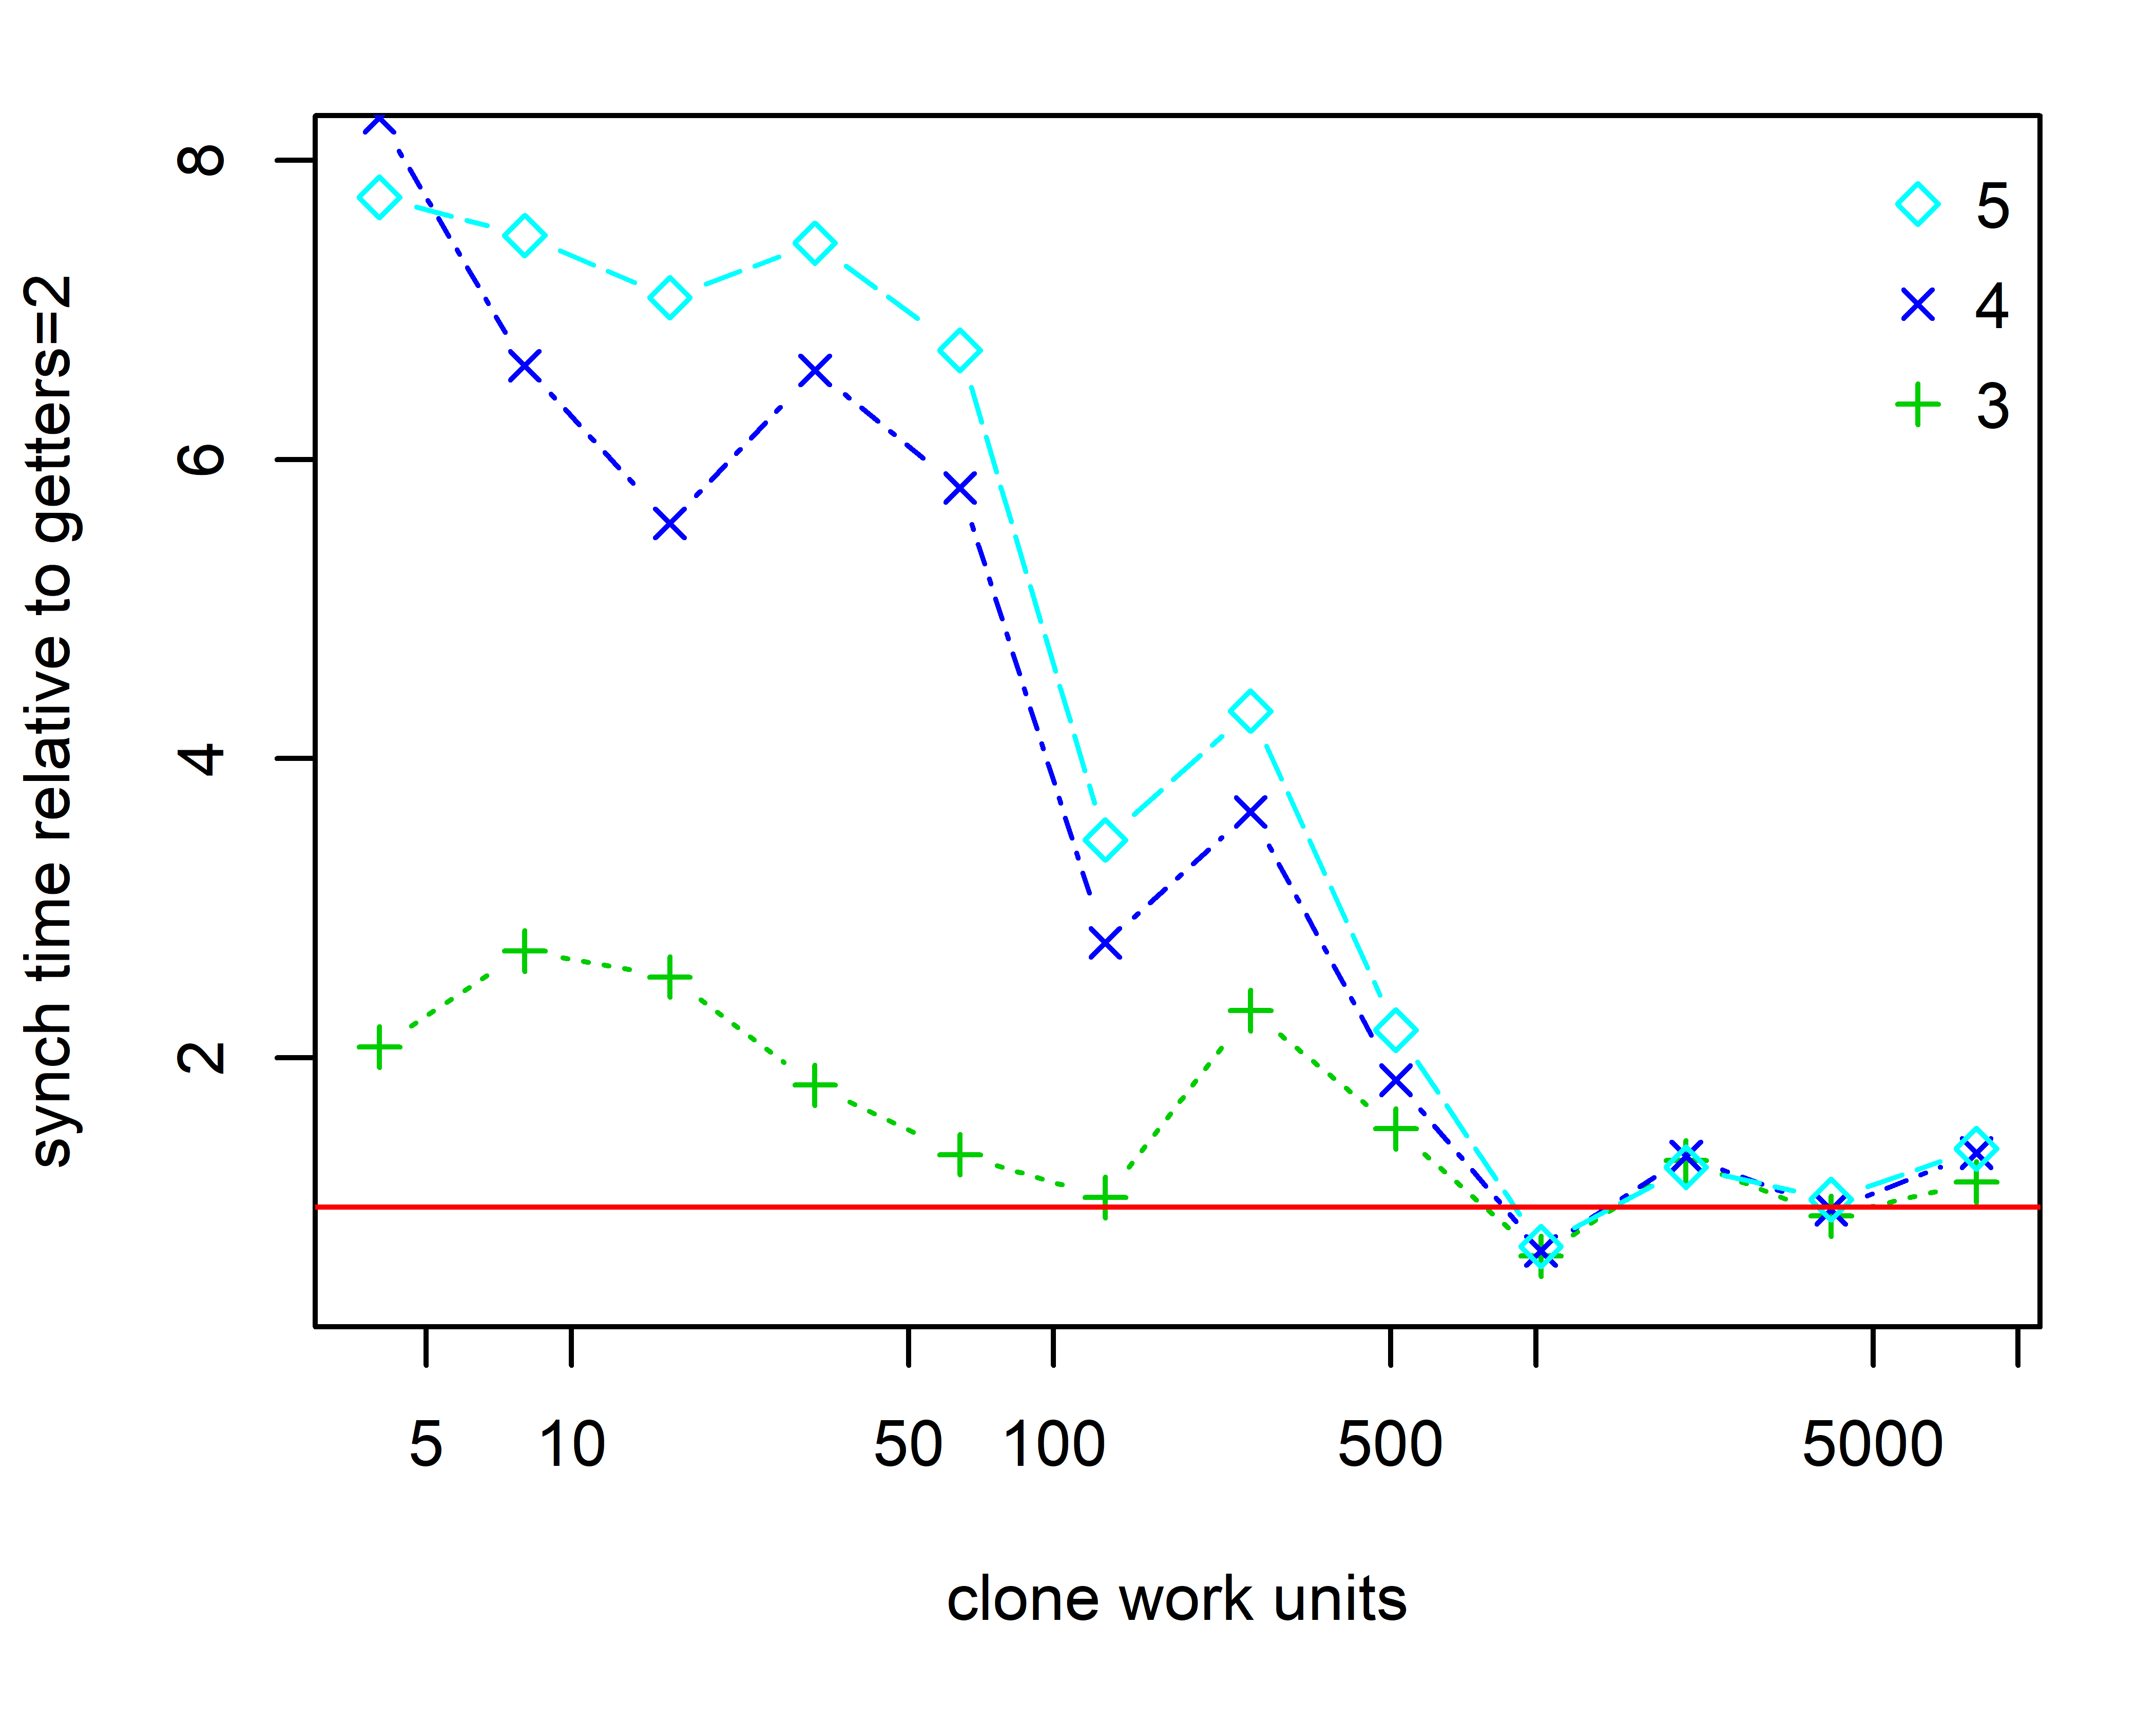
\includegraphics[width=0.67\textwidth]{experiments/clone_compete_2.png}
	\caption[TODO]{TODO.}
	\label{fig:clone_compete_3}
\end{figure}


From before we saw that copying is more effective than cloning. its a vital optimization. lastly we try get a handle on the performance characteristics by varying the shallow object size (the only thing that matters)
Figure~\ref{fig:simo_copy} shows how it works with a multithreaded replicator connector. 
observe how the time taken increases with larger data as less fits in the cache. observe that the contention on the atomics (hardware locks) causes there to be superlinear overhead?? not sure what that's about. but observe that it does go down the larger the data becomes, showing that getters are able to get more effectively in parallel
\begin{figure}
	\centering
	\makebox[\textwidth][c]{
		\begin{subfigure}[b]{0.63\textwidth}
			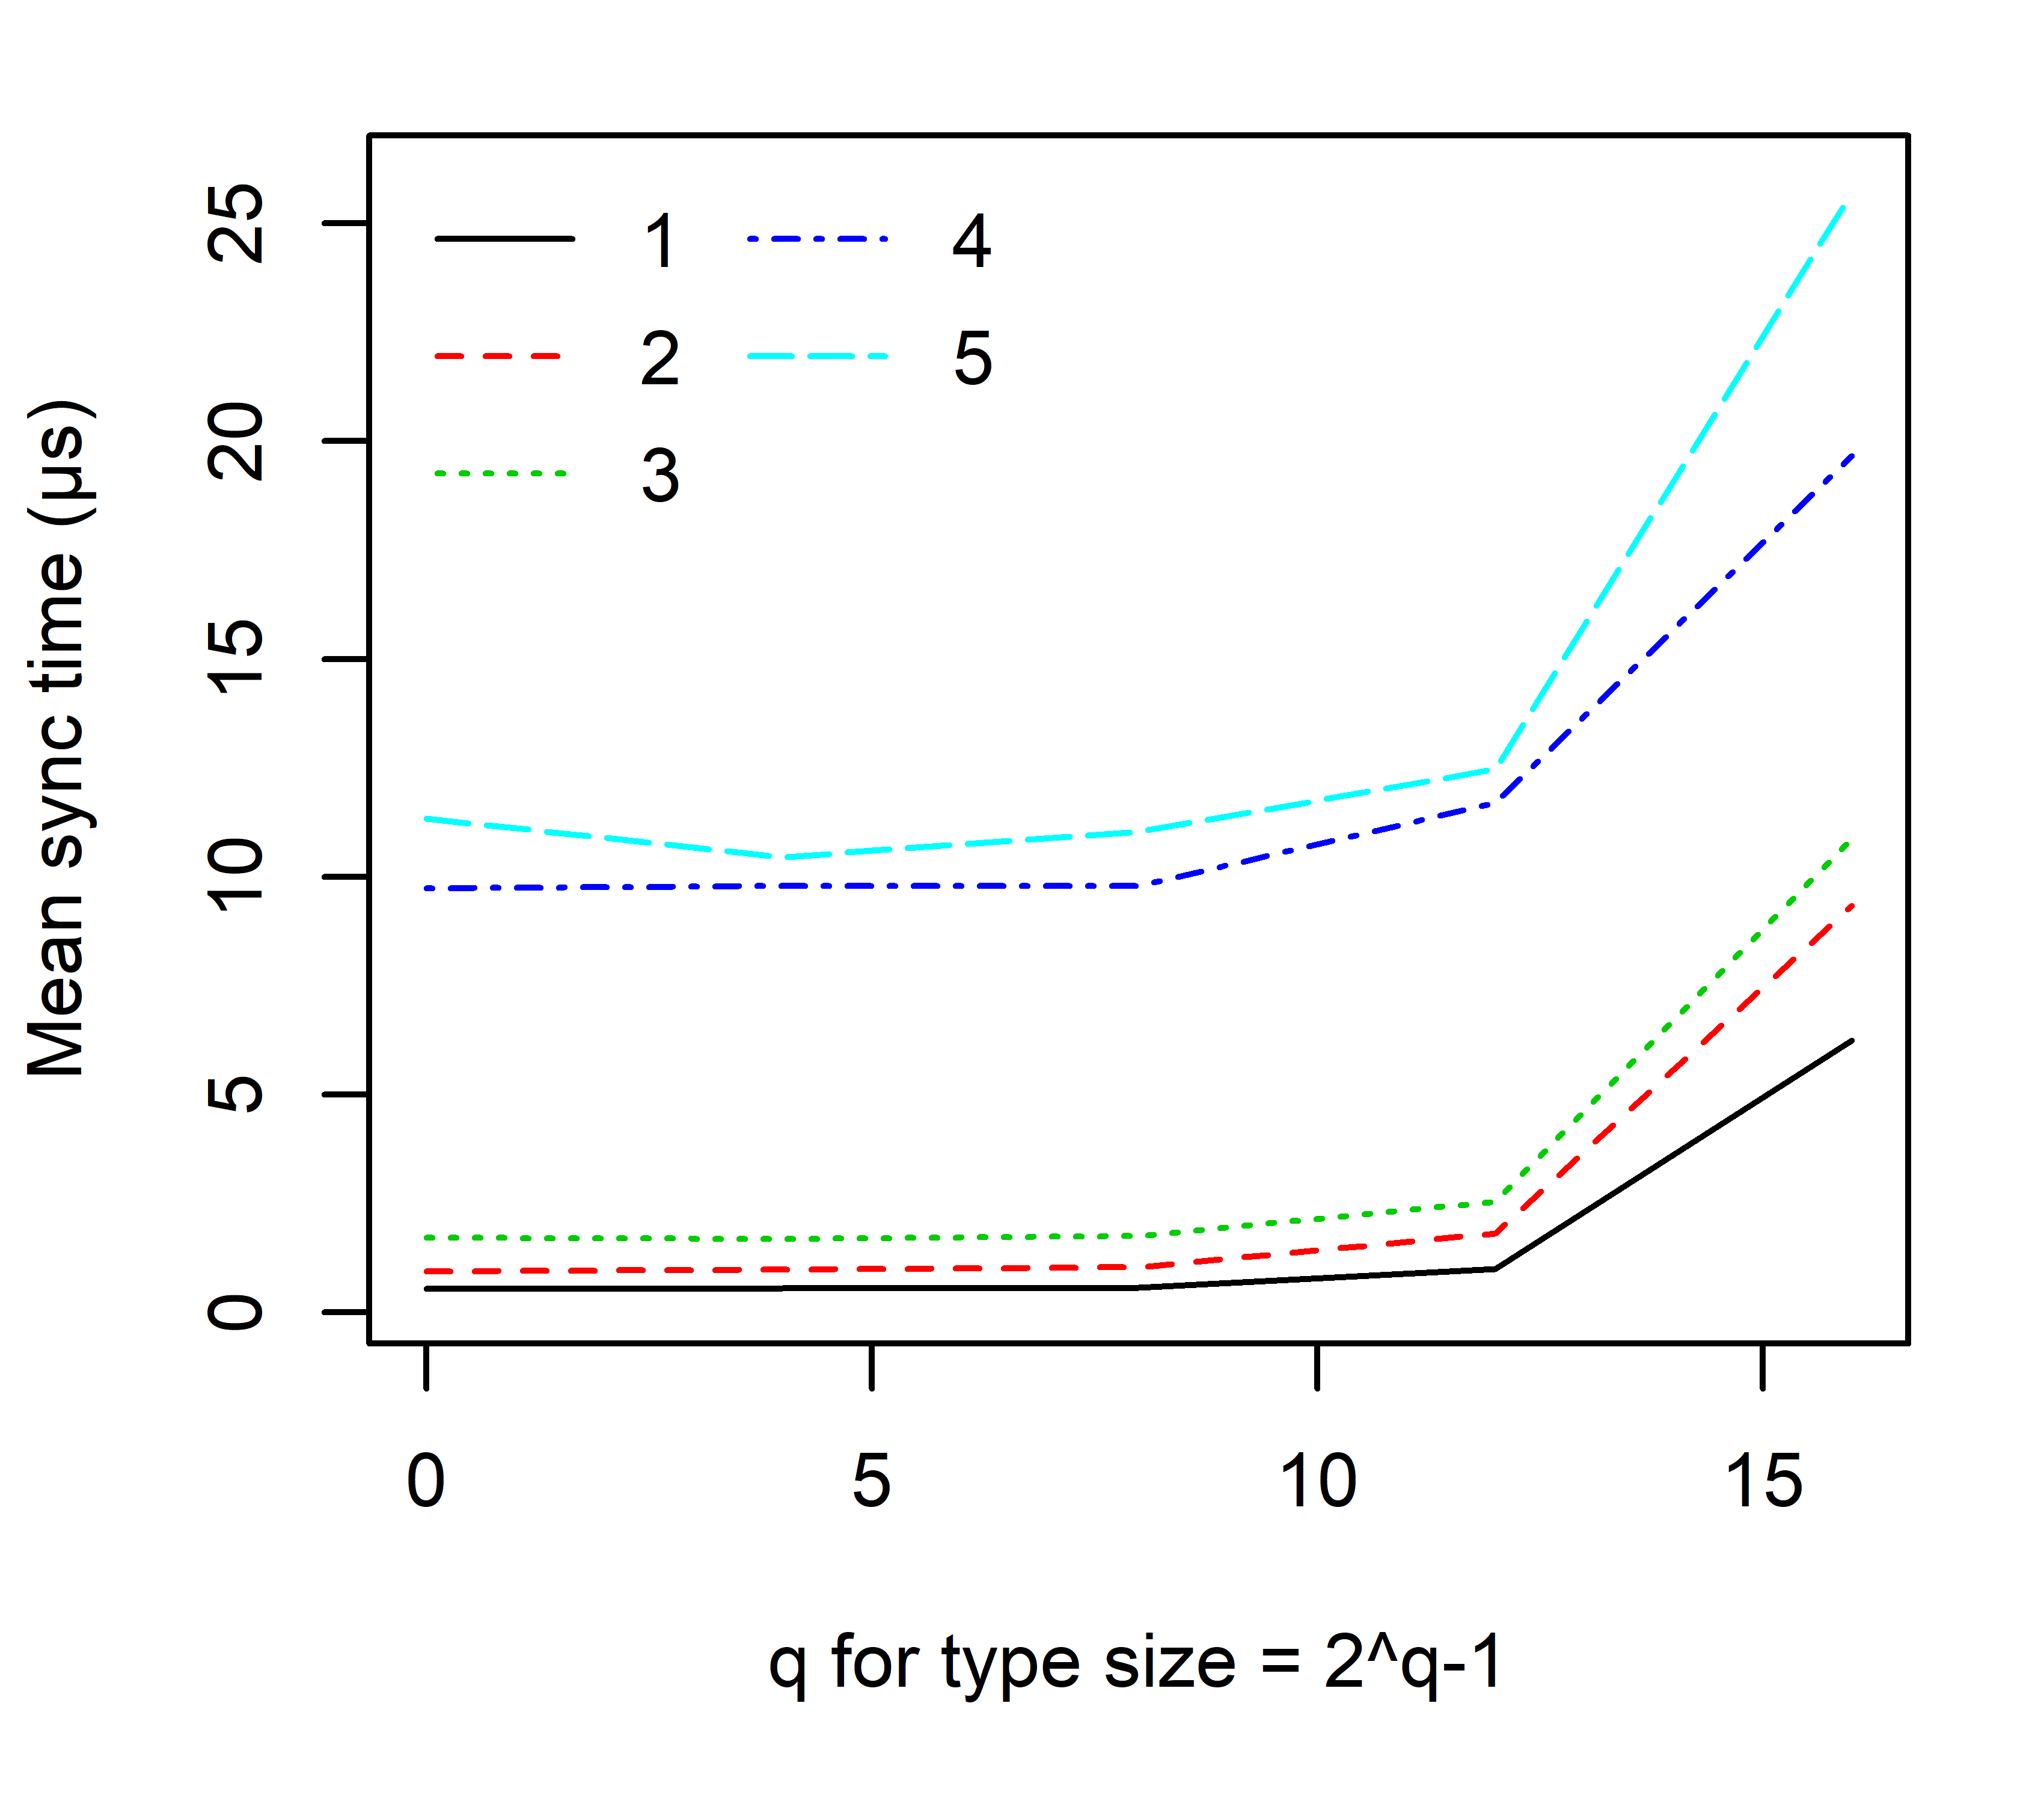
\includegraphics[width=\textwidth]{experiments/simo_copy_0.png}
			\caption{}
			\label{fig:simo_copy_0}
		\end{subfigure}%
		\begin{subfigure}[b]{0.63\textwidth}
			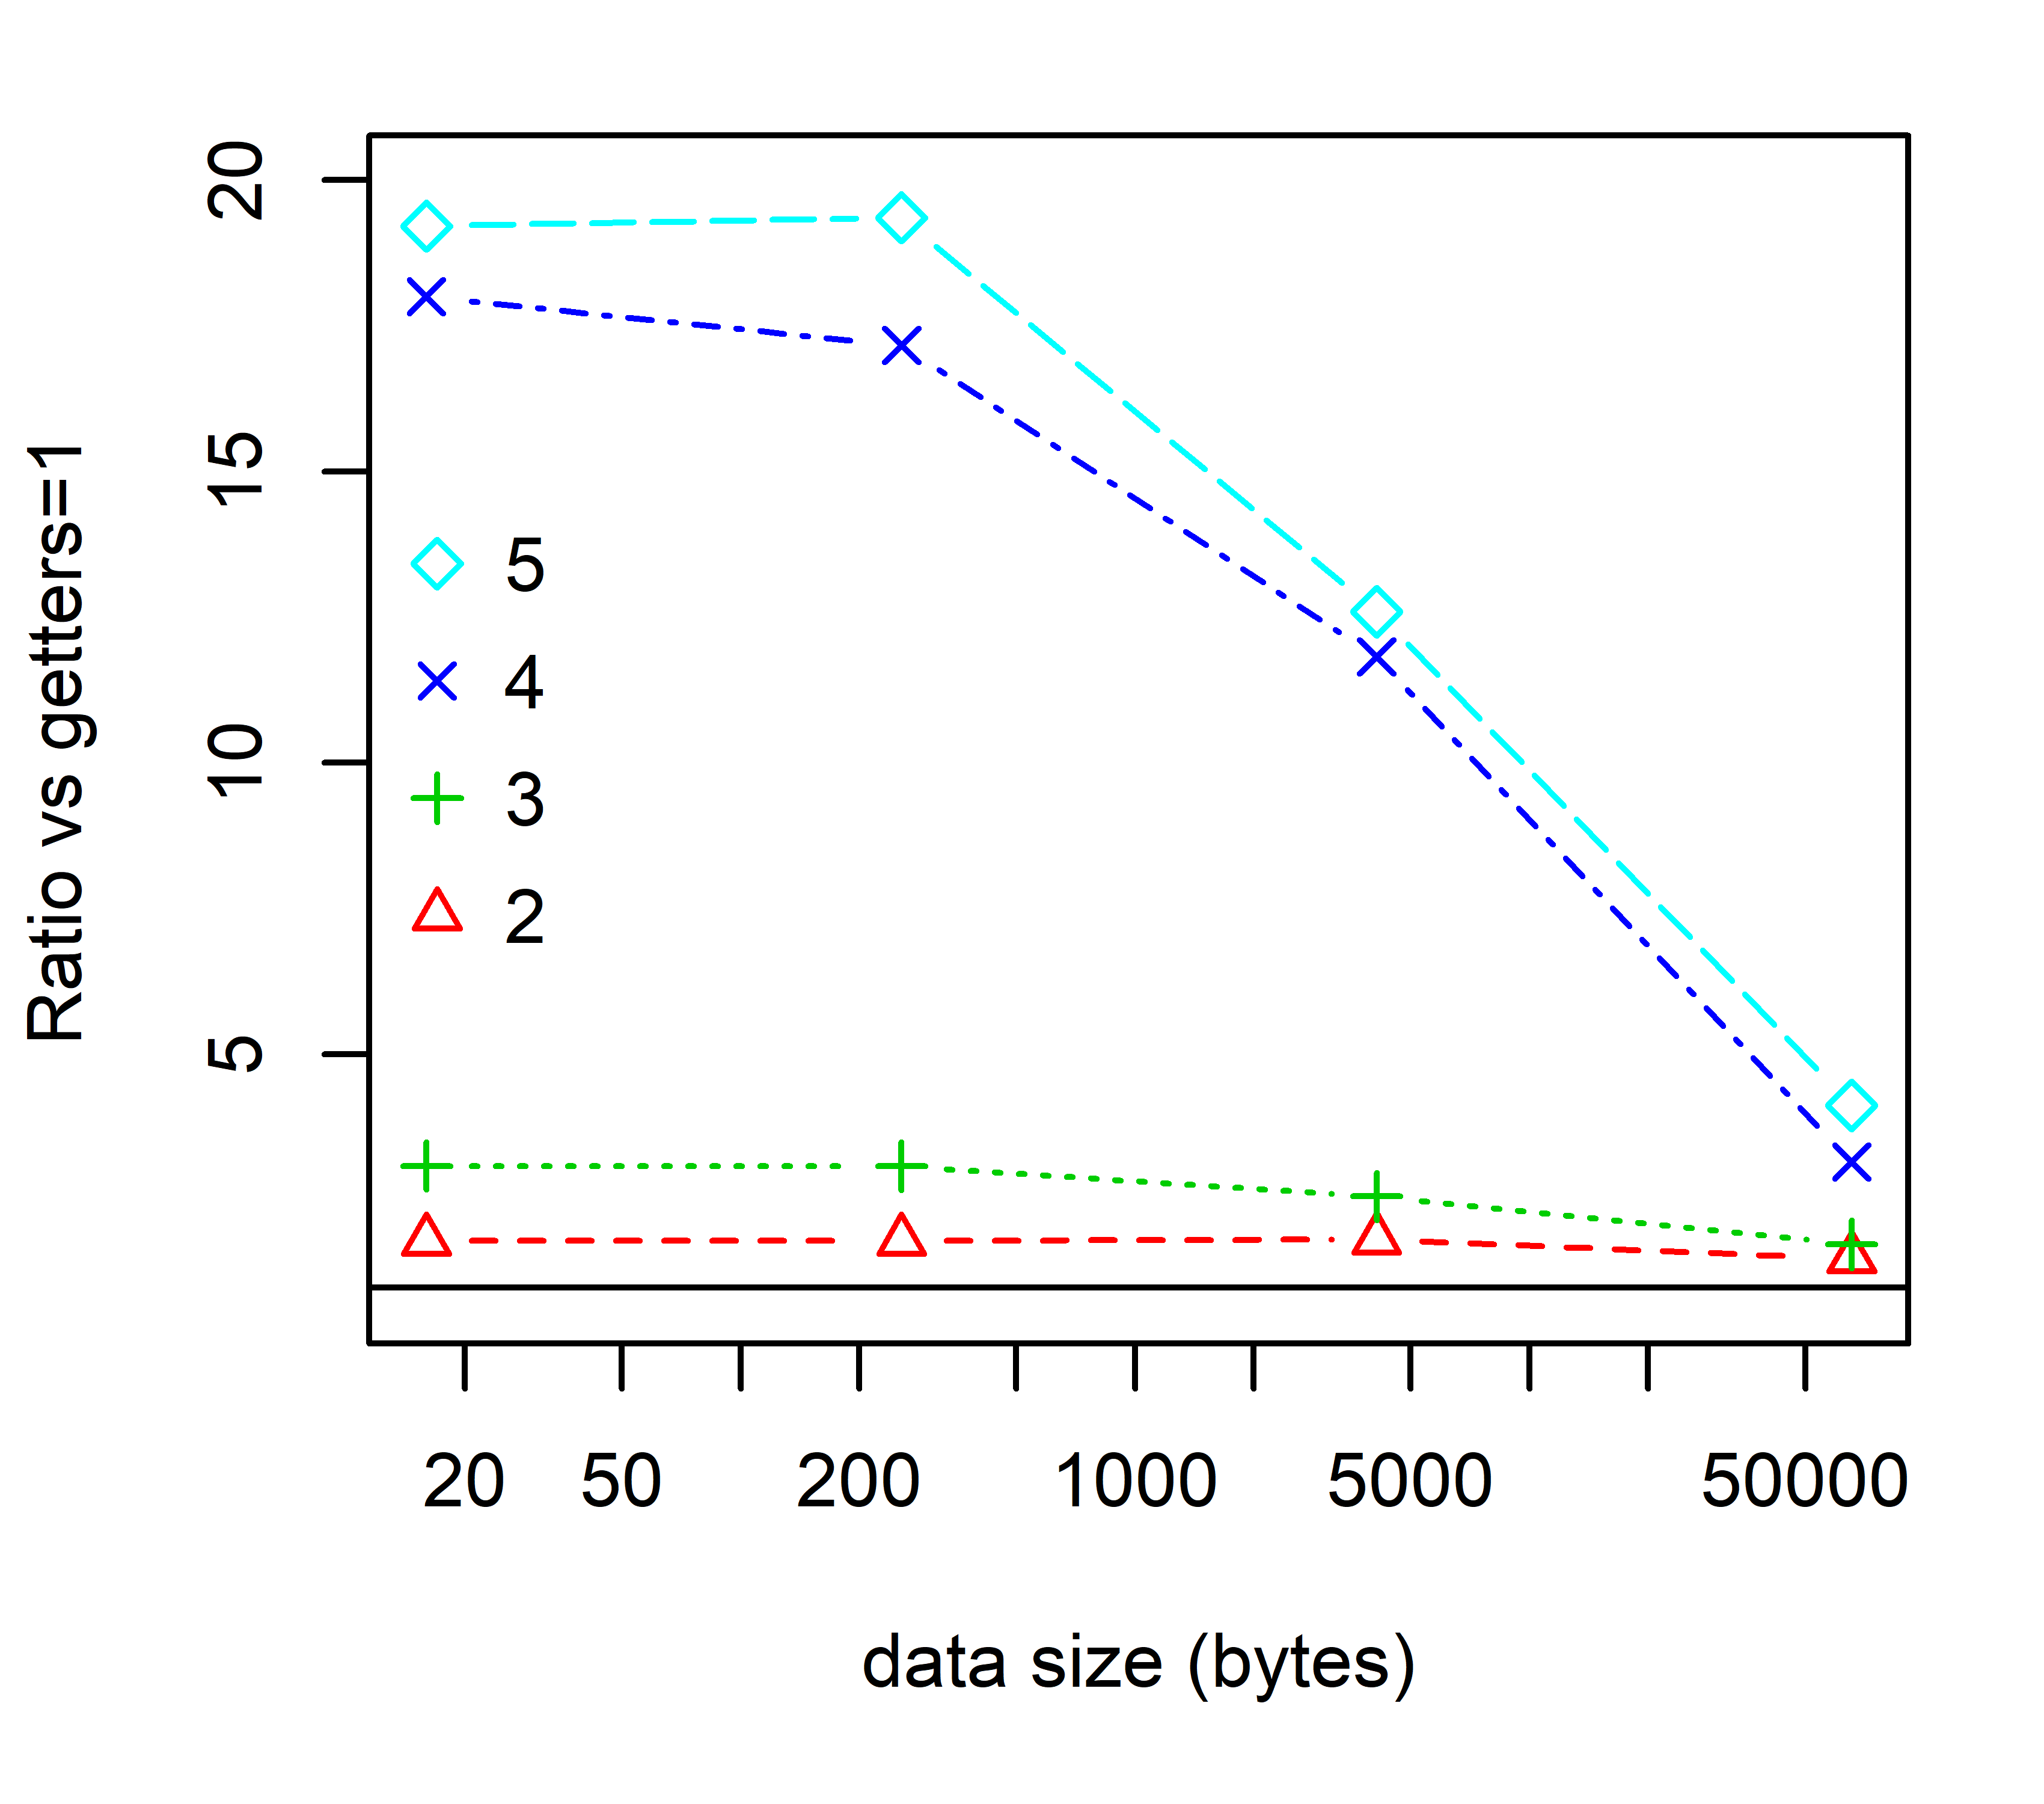
\includegraphics[width=\textwidth]{experiments/simo_copy_1.png}
			\caption{}
			\label{fig:simo_copy_1}
		\end{subfigure}%
	}
	\caption[TODO]{TODO.}
	\label{fig:simo_copy}
\end{figure}

